
\chapter{Results}
\label{ch:Results}
%Deep thoughts go here.
\section{Uncertainties}
\section{Statistical Treatment of Results}
\section{Limit on Branching Ratio t$\rightarrow$q$\gamma$}



%
%%%%%%%%%%%%%%%%%%%%%%%%%%%%%%%%%%%%%%%%%%%%%%%%
%%%%%%%%%%%%%                                                                                                   %%%%%%%% 
%%%%%%%%%%%%%                           BEN                                                                  %%%%%%%% 
%%%%%%%%%%%%%                                                                                                   %%%%%%%% 
%%%%%%%%%%%%%%%%%%%%%%%%%%%%%%%%%%%%%%%%%%%%%%%%
%This chapter contains co-authored material from Ref.~\cite{Dijet2017}, written as part of the ATLAS Collaboration.
%\newline
%
%Figure~\ref{fig:Figure1} shows the observed \mjj~distribution for events passing the resonance selection.  The red line overlaying the data shows result of the sliding window fit across the entire spectrum, while the second panel shows the significances of the data-fit discrepancies in each bin.  Two sample mass points of the $q*$ benchmark model are shown at 10$\times$ their predicted cross-section to illustrate the shape of a possible excess, and to make the points visible above the data distribution.
%
%The BumpHunter algorithm quantifies the statistical significance of any localized excess in the \mjj distribution.  The algorithm compares the binned \mjj~distribution of the data to the fitted background estimate, considering contiguous mass intervals in all possible locations, from a width of two bins to a width of half of the distribution. For each interval in the scan, it computes the significance of any excess found. The algorithm identifies the interval 4326–4595\,GeV, indicated by the two vertical lines in Figure~\ref{fig:Figure1}, as the most discrepant interval in the signal region. The global significance of this outcome is evaluated using the ensemble of possible outcomes across all intervals scanned, by applying the algorithm to pseudo-data samples drawn randomly from the background fit. Without including systematic uncertainties, the probability that fluctuations of the background model would produce an excess at least as significant as the one observed in the data anywhere in the distribution (the BumpHunter probability) is 0.63. Thus, there is no evidence of a localized contribution to the mass distribution from BSM phenomena.
%
%The 3rd panel of Figure~\ref{fig:Figure1} shows a comparison of the data spectrum to the prediction of Pythia8 simulated QCD processes, with next-to-leading order and electroweak correction factors applied, along with the band of uncertainty due to the jet energy scale calibration.  This comparison is not used for any of the fits or limits, but is only to demonstrate that the spectrum is in agreement with theory expectations.
%
%Figure~\ref{fig:Figure2} shows the observed \mjj~distribution for events passing the wider $W*$ resonance selection.  The same interval is identified as the most discrepant, and the BumpHunter probability is 0.83, meaning no evidence of an excess in the invariant mass distribution.
%
%\begin{figure}[]
%	\centering
%	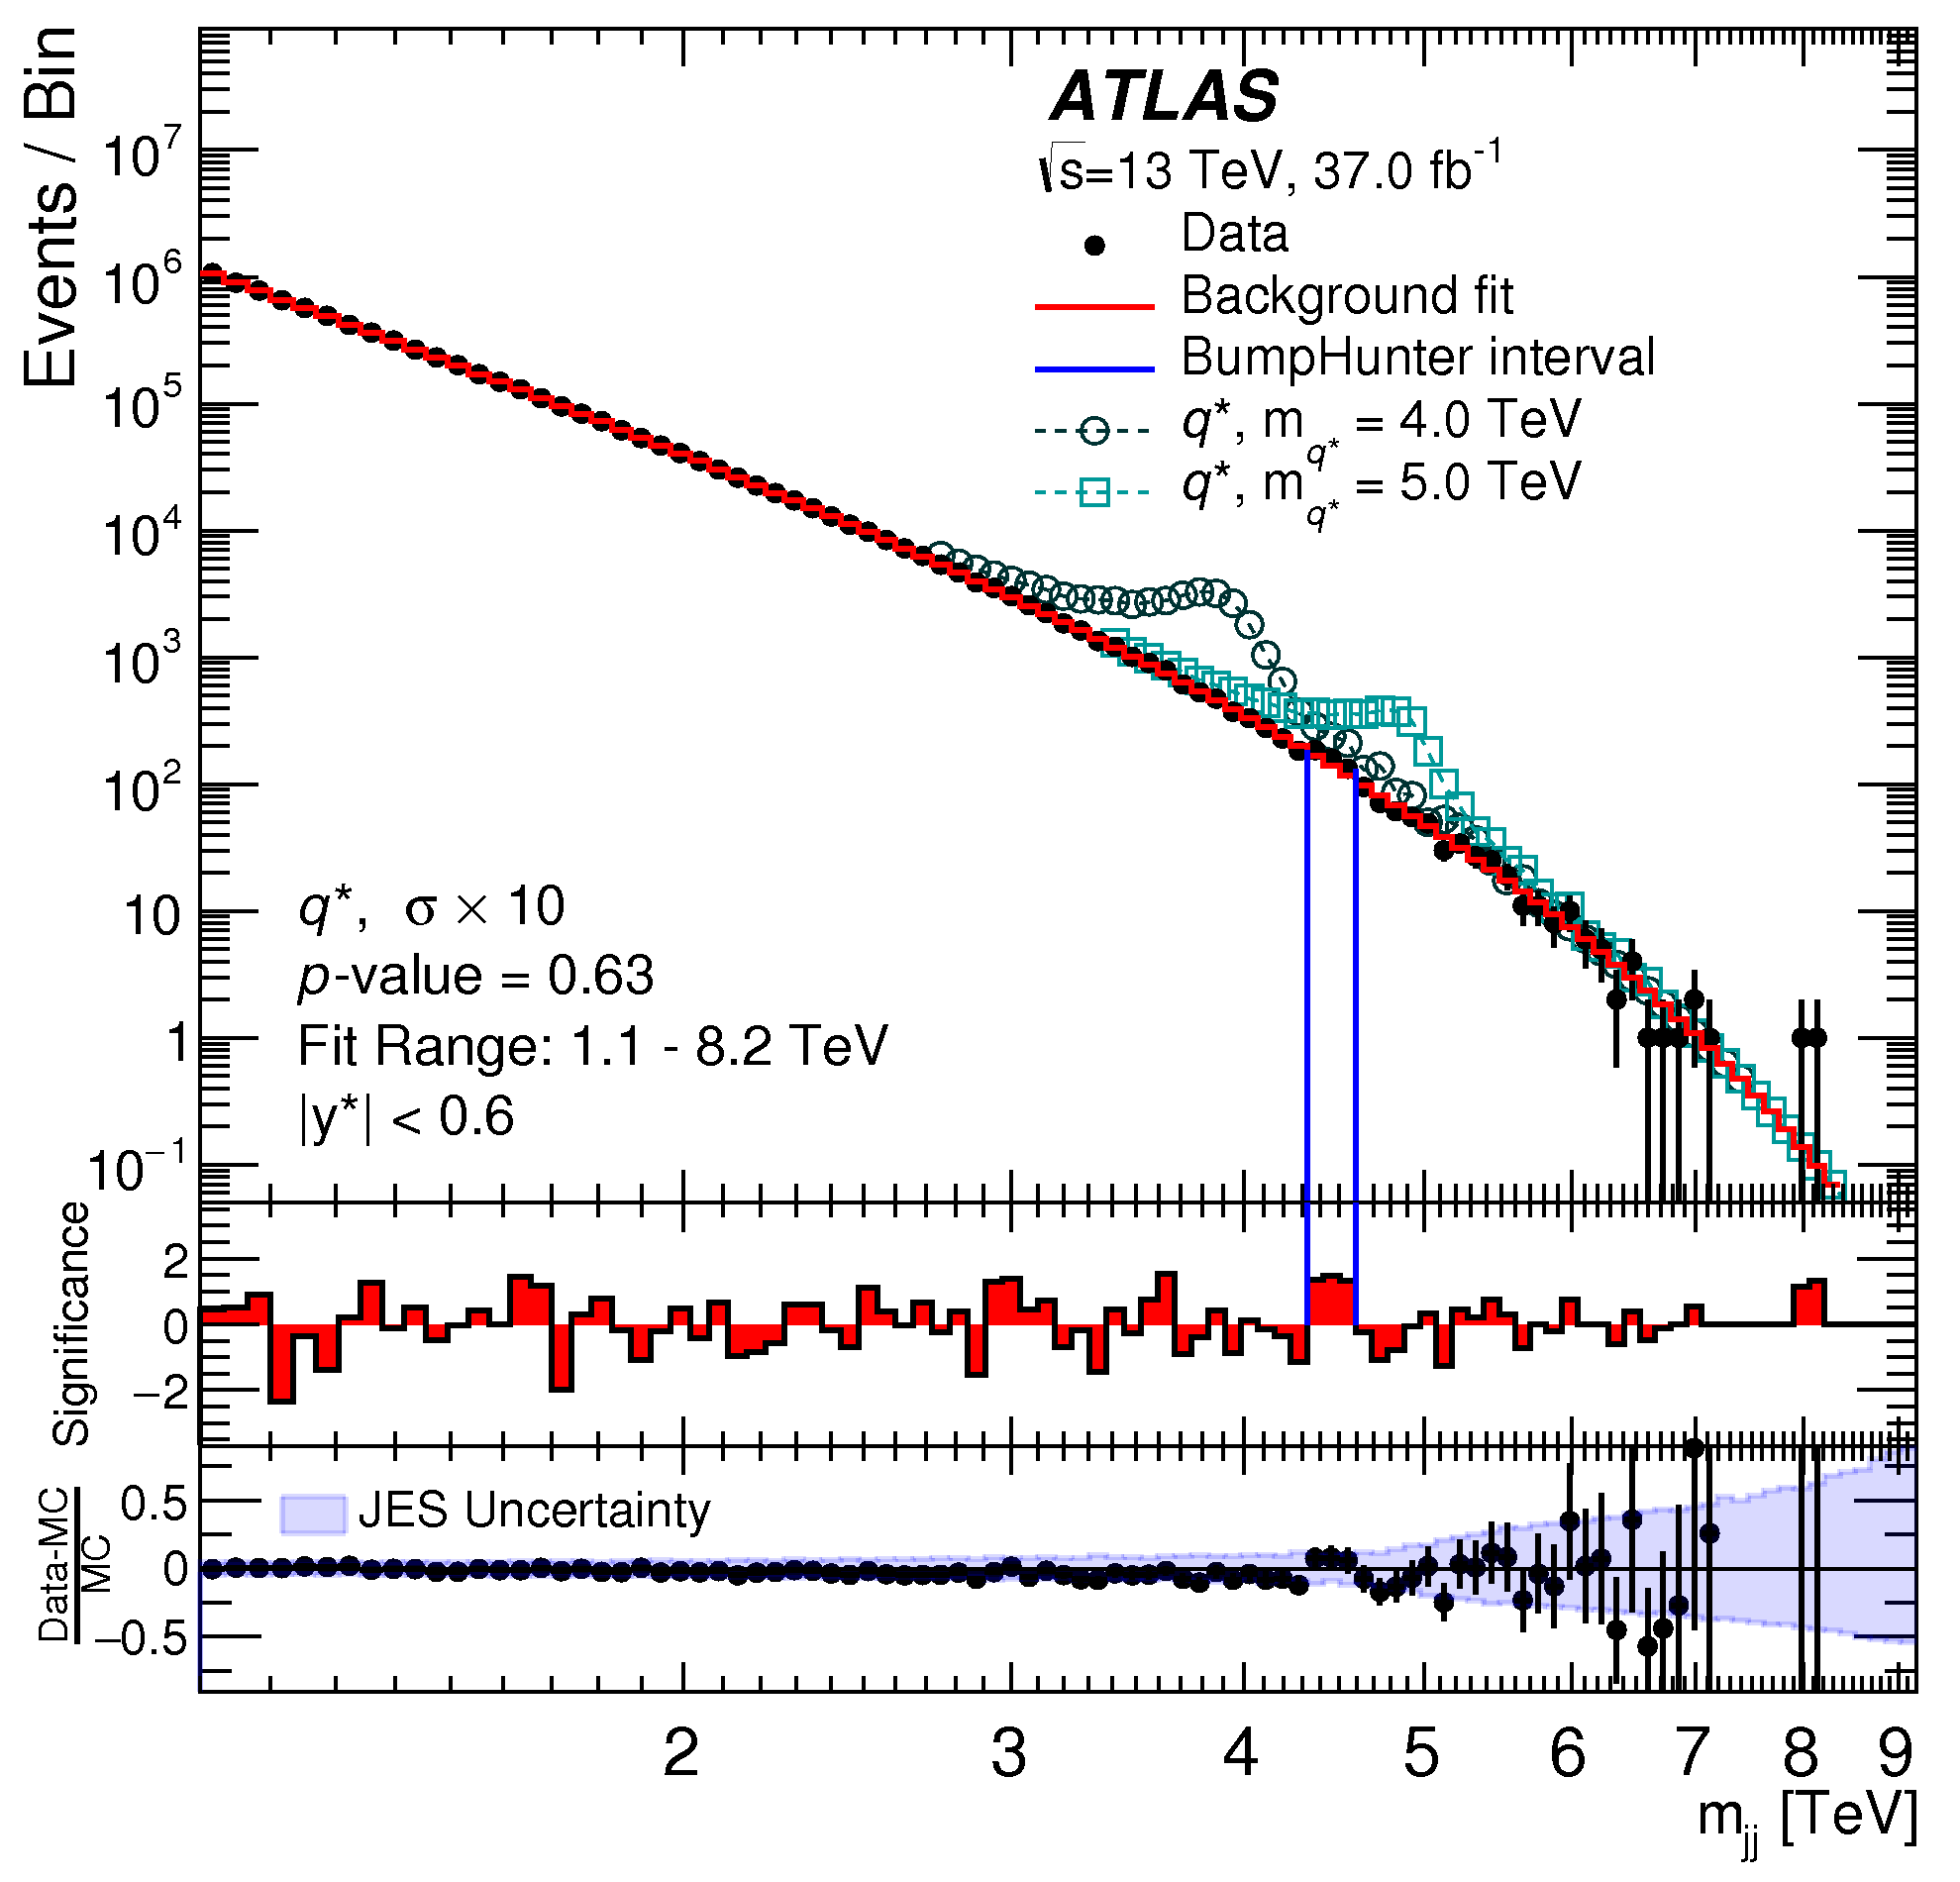
\includegraphics[width=0.8\columnwidth]{figures/Results/Figure1.png}
%	\caption{ The reconstructed dijet mass distribution \mjj (filled points) is shown for events with \pt $>$ 440 (60)\,GeV for the leading (subleading) jet in the resonance $y^*<0.6$ signal region. The solid line depicts the background prediction from the sliding-window fit. The vertical lines indicate the most discrepant interval identified by the BumpHunter algorithm, for which the p-value is 0.63. The middle panel shows the bin-by-bin significances of the data–fit differences, considering only statistical uncertainties. The lower panel shows the relative differences between the data and the prediction of Pythia 8 simulation of QCD processes, corrected for NLO and electroweak effects, and is shown purely for comparison. The shaded band denotes the experimental uncertainty in the jet energy scale calibration.}
%	\label{fig:Figure1}
%\end{figure}
%
%\begin{figure}[]
%	\centering
%	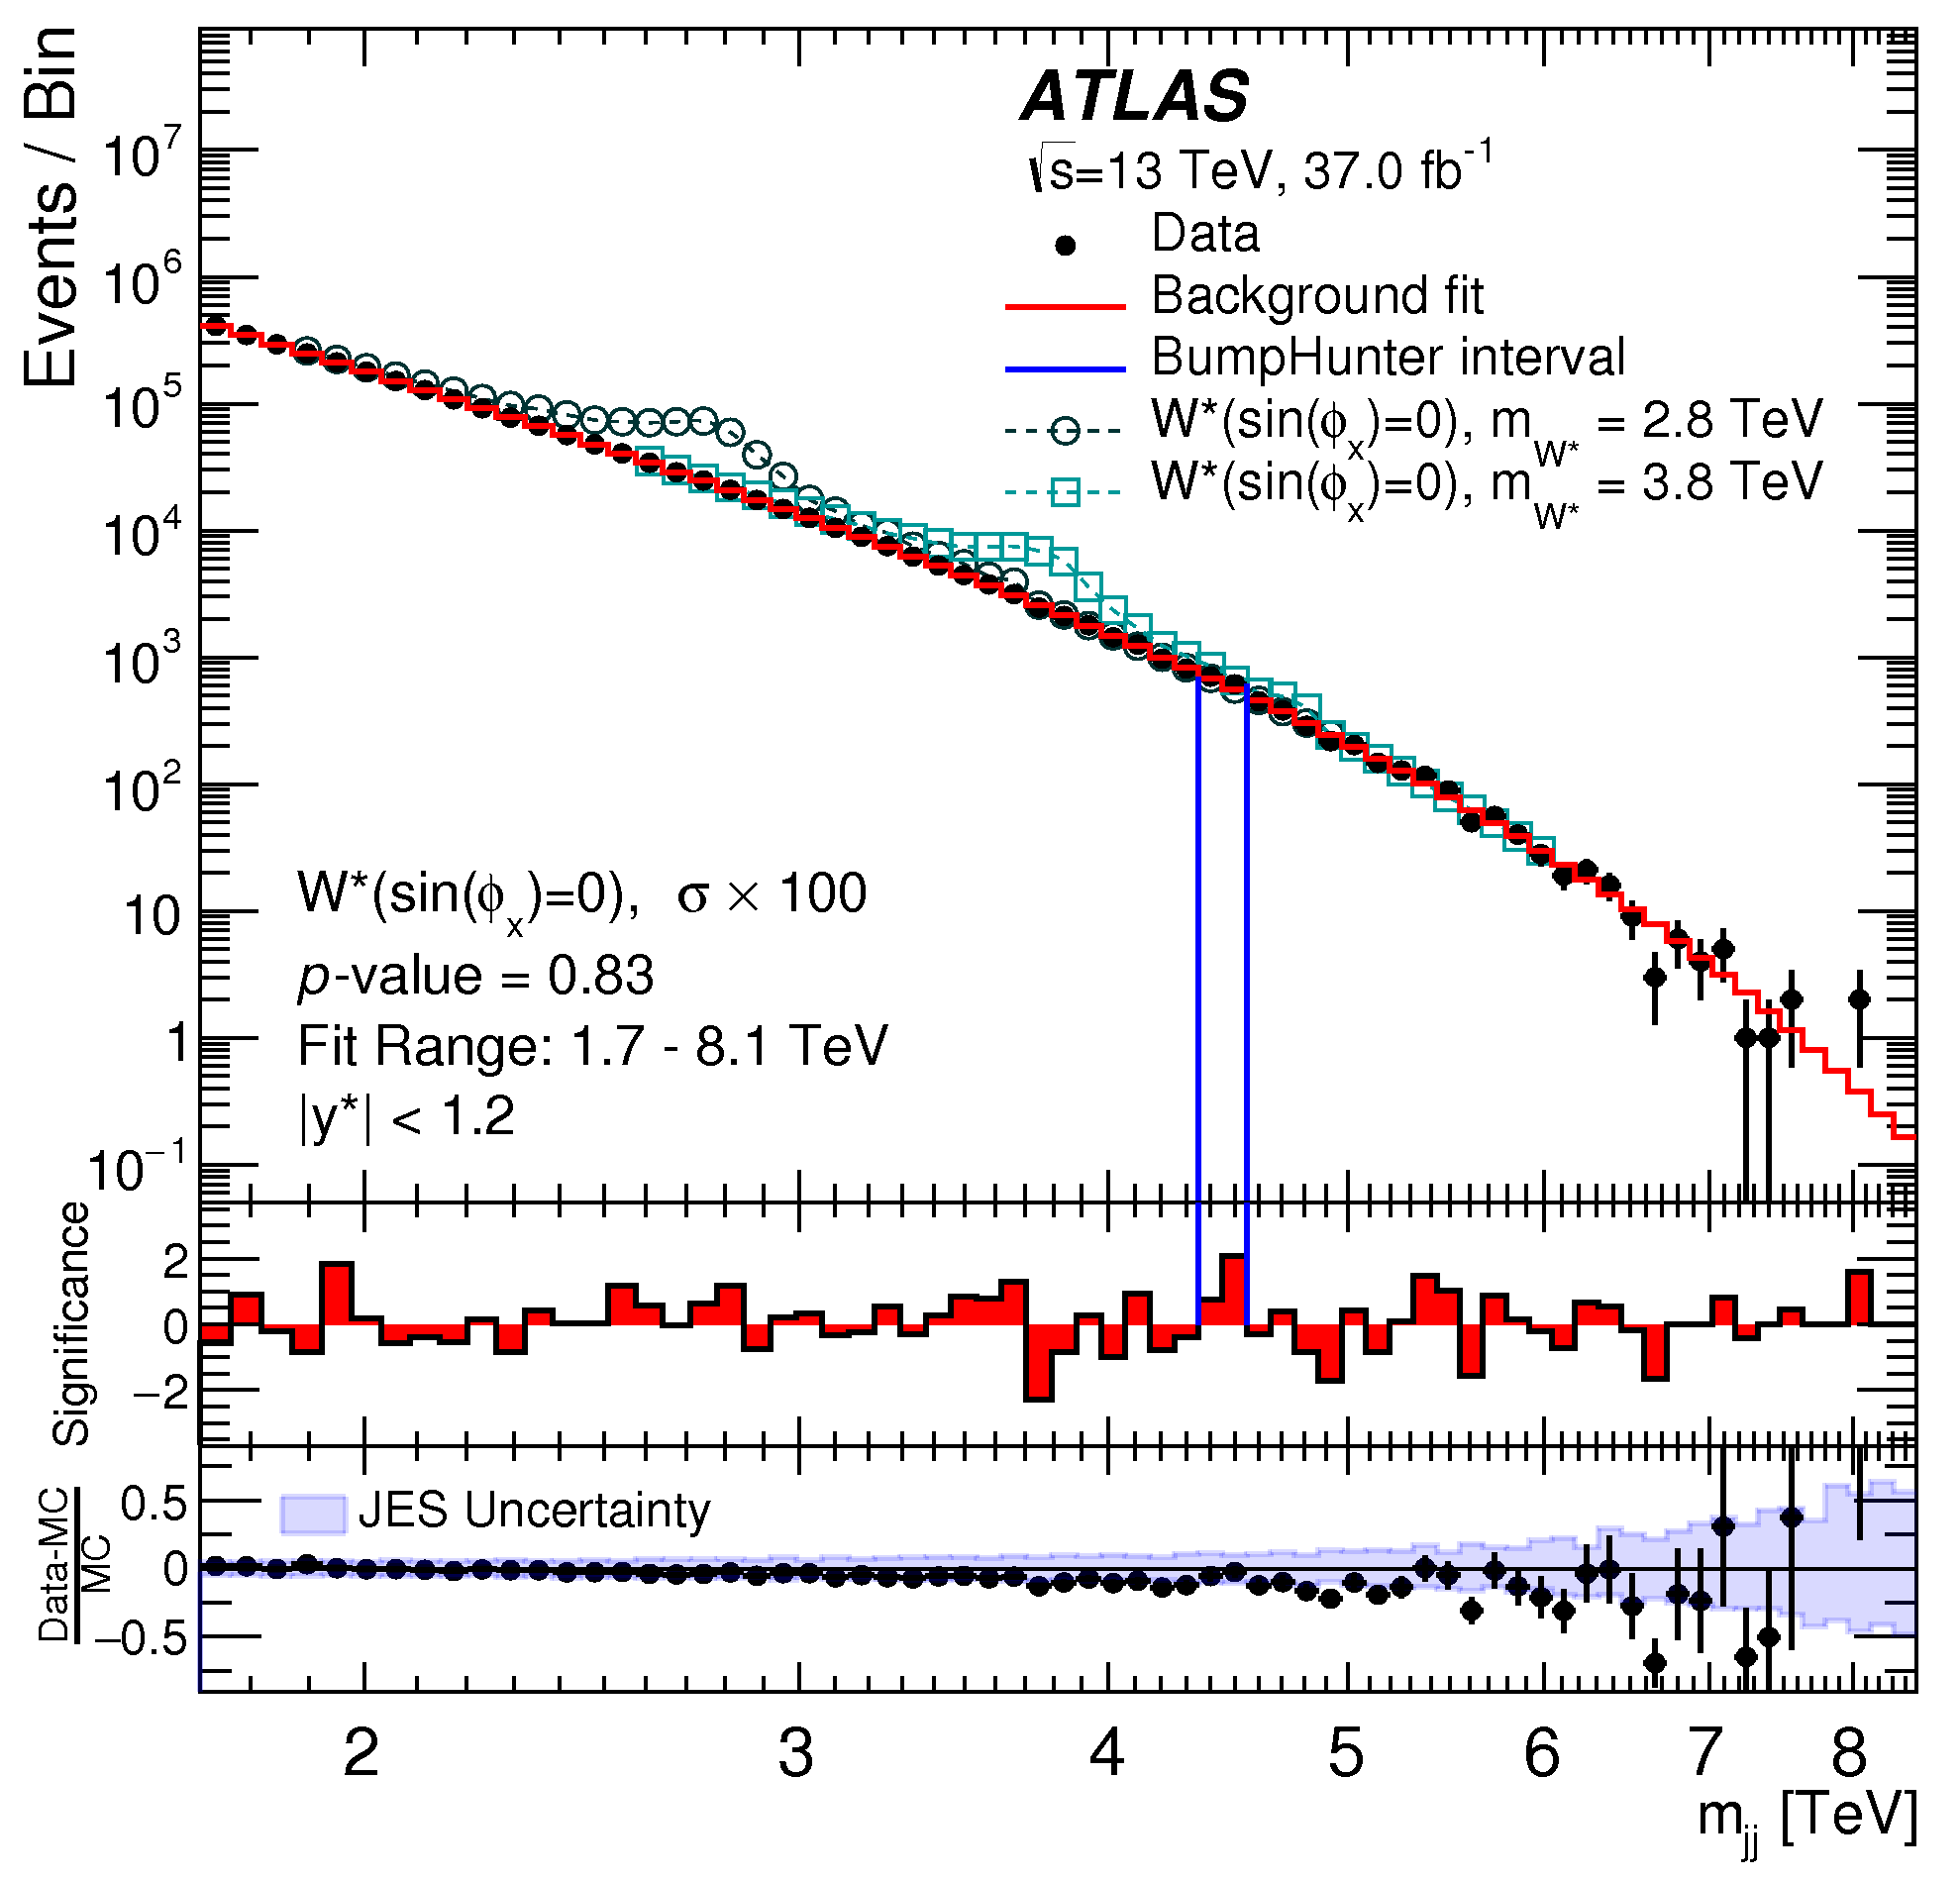
\includegraphics[width=0.8\columnwidth]{figures/Results/Figure2.png}
%	\caption{ The reconstructed dijet mass distribution \mjj (filled points) is shown for events with \pt $>$ 440 (60)\,GeV for the leading (subleading) jet in the $W*$ resonance $y^*<1.2$ signal region. The solid line depicts the background prediction from the sliding-window fit. The vertical lines indicate the most discrepant interval identified by the BumpHunter algorithm, for which the p-value is 0.83. The middle panel shows the bin-by-bin significances of the data–fit differences, considering only statistical uncertainties. The lower panel shows the relative differences between the data and the prediction of Pythia 8 simulation of QCD processes, corrected for NLO and electroweak effects, and is shown purely for comparison. The shaded band denotes the experimental uncertainty in the jet energy scale calibration.}
%	\label{fig:Figure2}
%\end{figure}
%
%The highest-mass event observed in the dataset is 8.12\,TeV and is shown in figure~\ref{fig:LargestEvent}.  Energy deposits in the EM (green) and hadronic (red) calorimeters are indicated by the bars radiating outward from the detector.  The white panels in the outside of the detector denote hits in the muon system, indicating that the energy for this event punched through the calorimeter system.
%
%\begin{figure}[ht!]
%	\centering
%	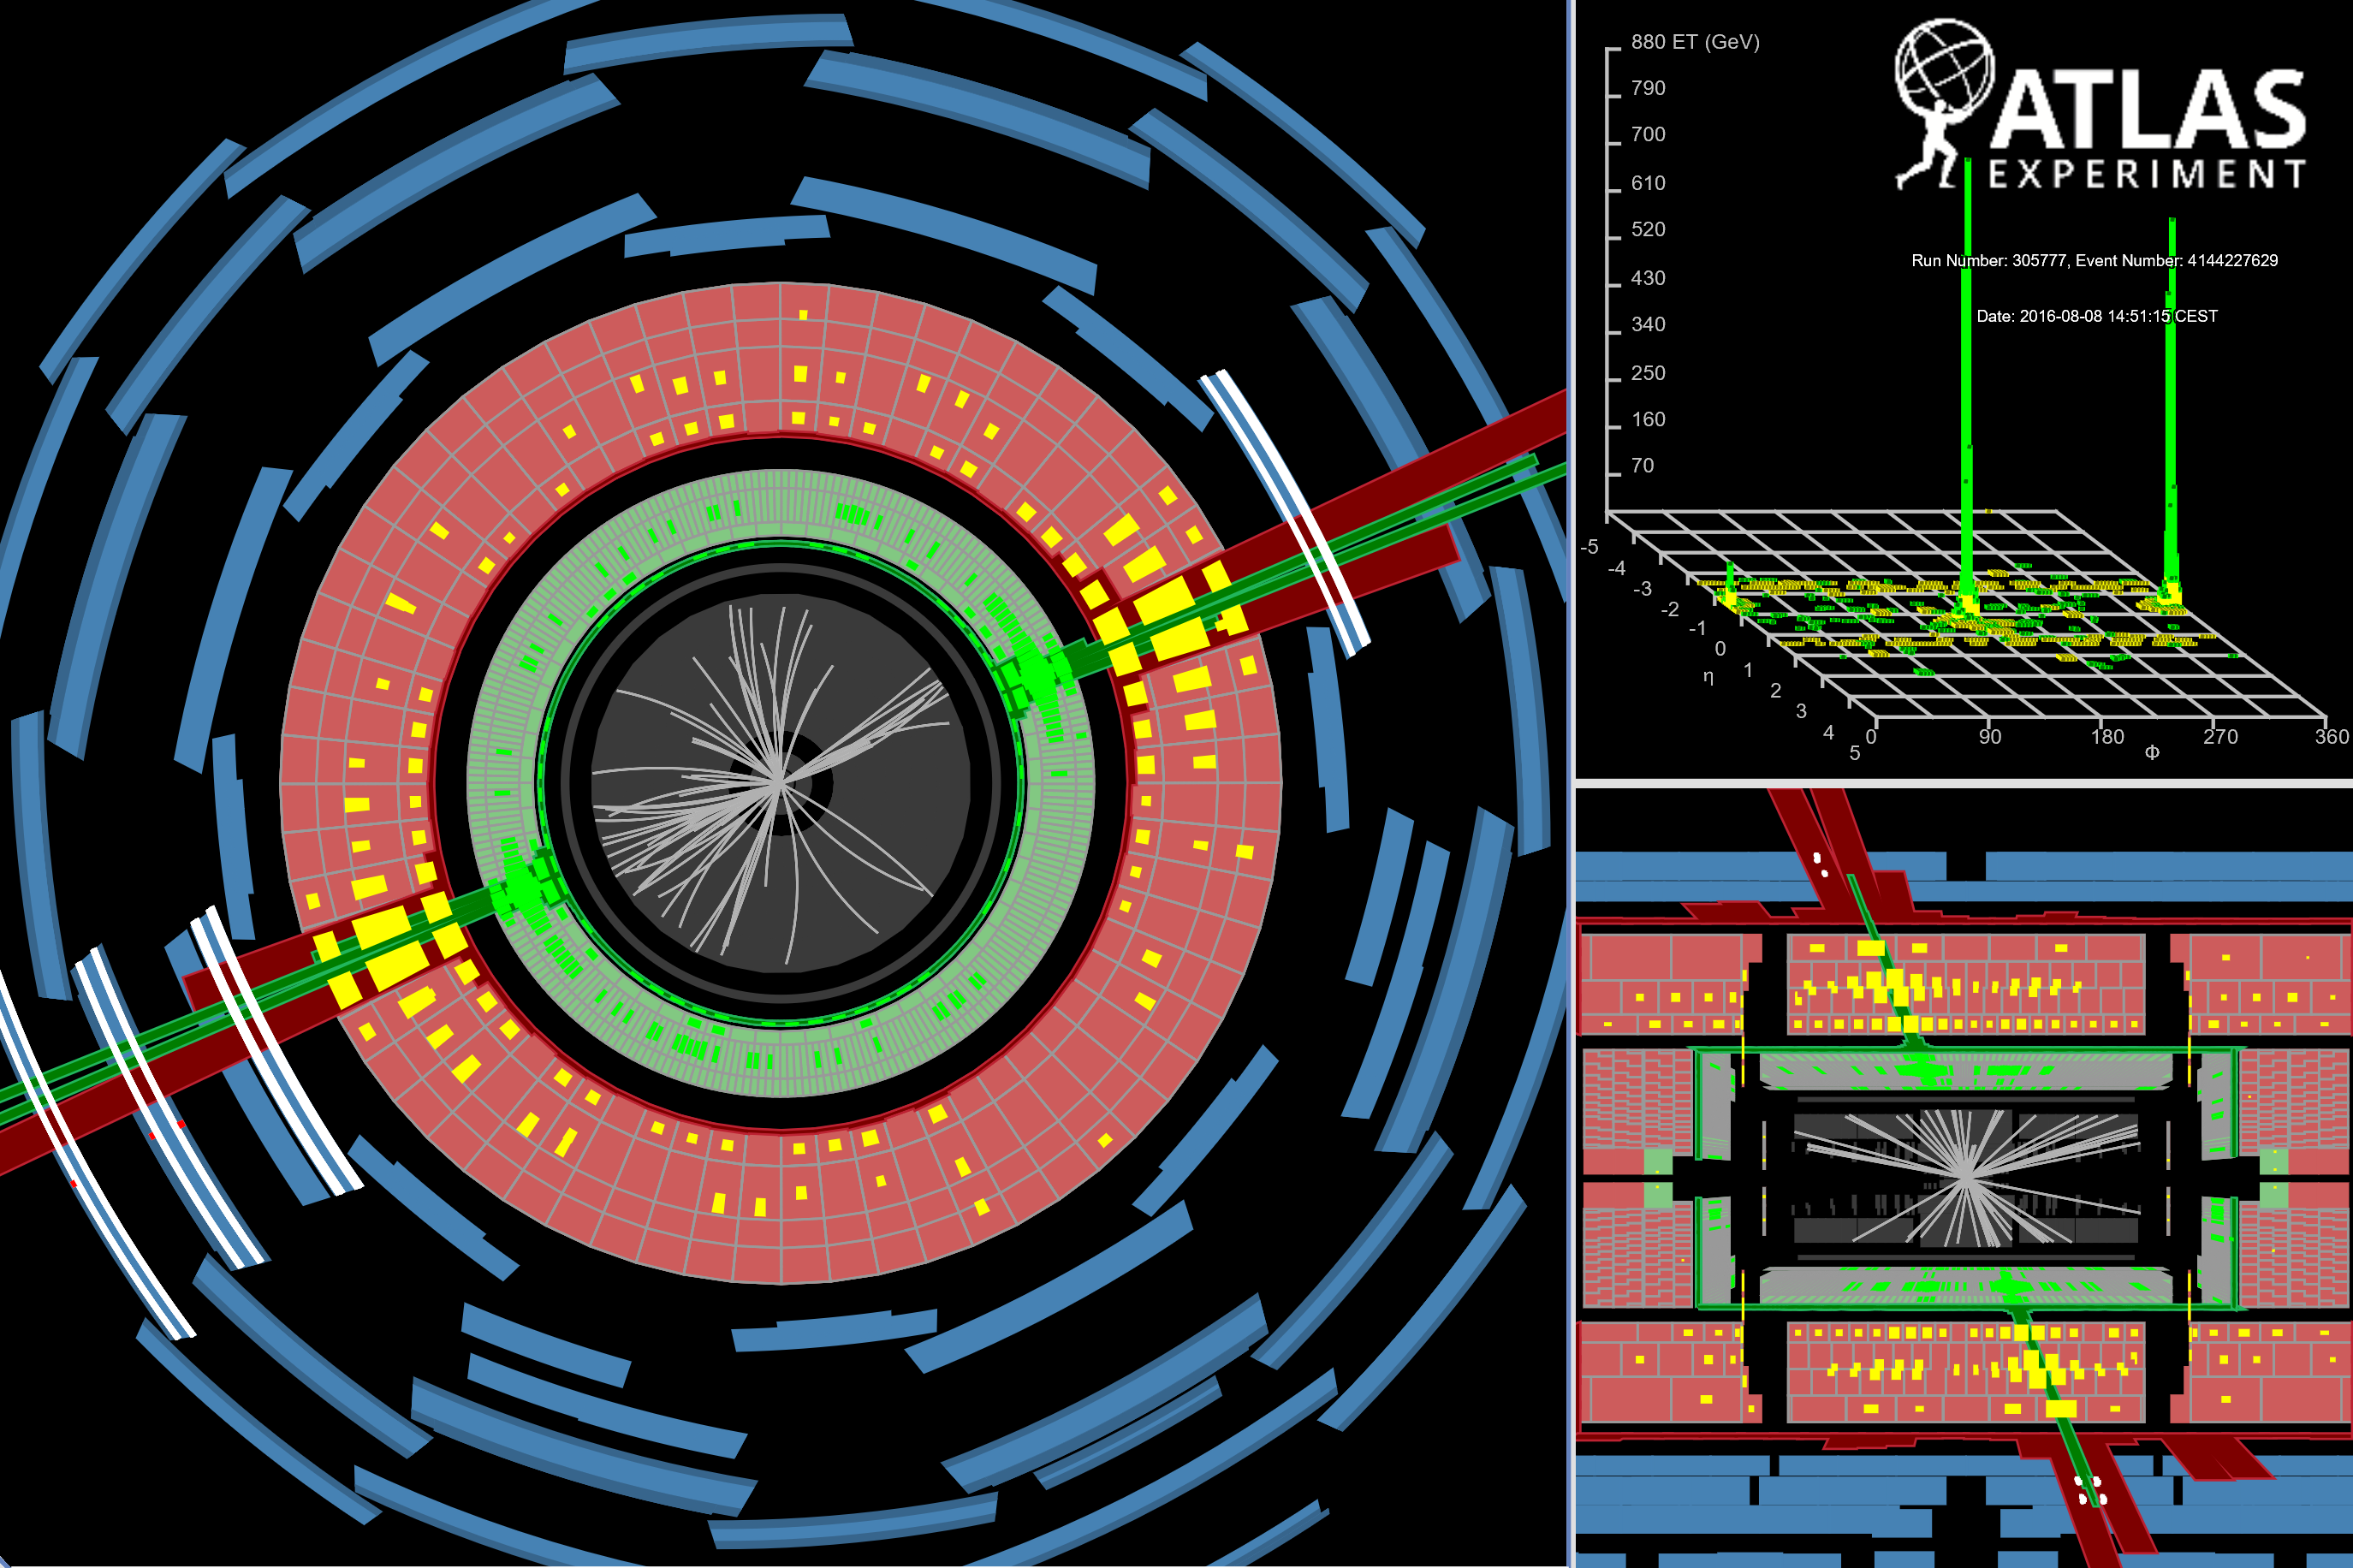
\includegraphics[width=\columnwidth]{figures/Results/LargestEvent.png}
%	\caption{The highest mass dijet event observed in the 2015+2016 dataset.  It has an invariant mass of 8.12\,TeV, and the two jets each have transverse momenta of 3.79\,TeV.}
%	\label{fig:LargestEvent}
%\end{figure}
%
%\section{Limit Setting and Bayes' Theorum}
%
%With no excess seen in the data, we can then used the observed spectrum to set limits on the presence of possible new physics.  This analysis uses several benchmark models and sets limits on their cross-sections.  Put another way, for each new physics model, at a given mass point, the largest number of events which would still be compatible with the background estimation is calculated.  A Bayesian statistical approach using a flat, non-informative prior is used to set limits~\cite{Bayesian}, with all nuisance parameters accounted for in the marginalizaiton step of the procedure.  To calculate the final limits, the analysis uses a Markov Chain Monte Carlo (MCMC) method to perform the the numerical integration needed to combine the nuisance parameters.  This is implemented using the Bayesian Analysis Toolkit~\cite{BAT}, a package specifically designed for physics use.  
%
%In addition to reporting an upper limit on the presence of a signal in the observed data, an expected limit is created to provide context for determining the deviation between observation and the expected null hypothesis of no signal.  This is done by creating an ensemble of pseudo-datasets generated by Poisson-fluctuating the background prediction from the analysis, then calculating the upper limit for each pseudoexperiment using the same marginalization procedure as used for the data.  The resulting distribution is used to define a central expected value, along with $1\sigma$ and $2\sigma$ error bands. 
%
%\section{Uncertainties}
%
%The dijet analysis is relatively insensitive to many sources of uncertainty, including the negligible jet energy resolution uncertainty and no theoretical uncertainties on the background parameterization due to the direct fit to data.  Each source of systematic uncertainty is assigned is treated as a unique nuisance parameter, the treatment of which is described in the next section.
%
%\subsection{Jet Energy Scale Uncertainty}
%The full treatment of jet energy scale uncertainty involves 84 nuisance parameters, the bulk of which come from the bin-to-bin correlations of the various in-situ analyses (Z+jet, $\gamma$+jet, and multijet balance), along with terms covering the eta intercalibration, pile-up, and the behavior of high-\pt jets.  Taking into account all of these variations requires a considerable amount of computing power and is infeasible for this analysis.  Instead, the analysis uses the strongly reduced uncertainties provided by the JetETMiss combined performance group.  These reduced sets consist of a single eta intercalibration term and three additional nuisance parameters which are combinations of the other 83 parameters.  These parameters are reduced down in four different configurations, and the dataset is tested against all four configurations to determine if the final analysis observables are sensitive to jet correlations.  The final dijet spectrum showed negligible differences between strong reduction sets, and thus any one of them can be used without loss of sensitivity compared to the full set of nuisance parameters.
%For the dijet analysis, the uncertainty is dominated by whichever parameter contains the high-\pt term.  This uncertainty ranges from 1.5\% at low invariant mass to 3\% for masses above 4.5\,TeV.\
%\begin{figure}[ht!]
%	\centering
%	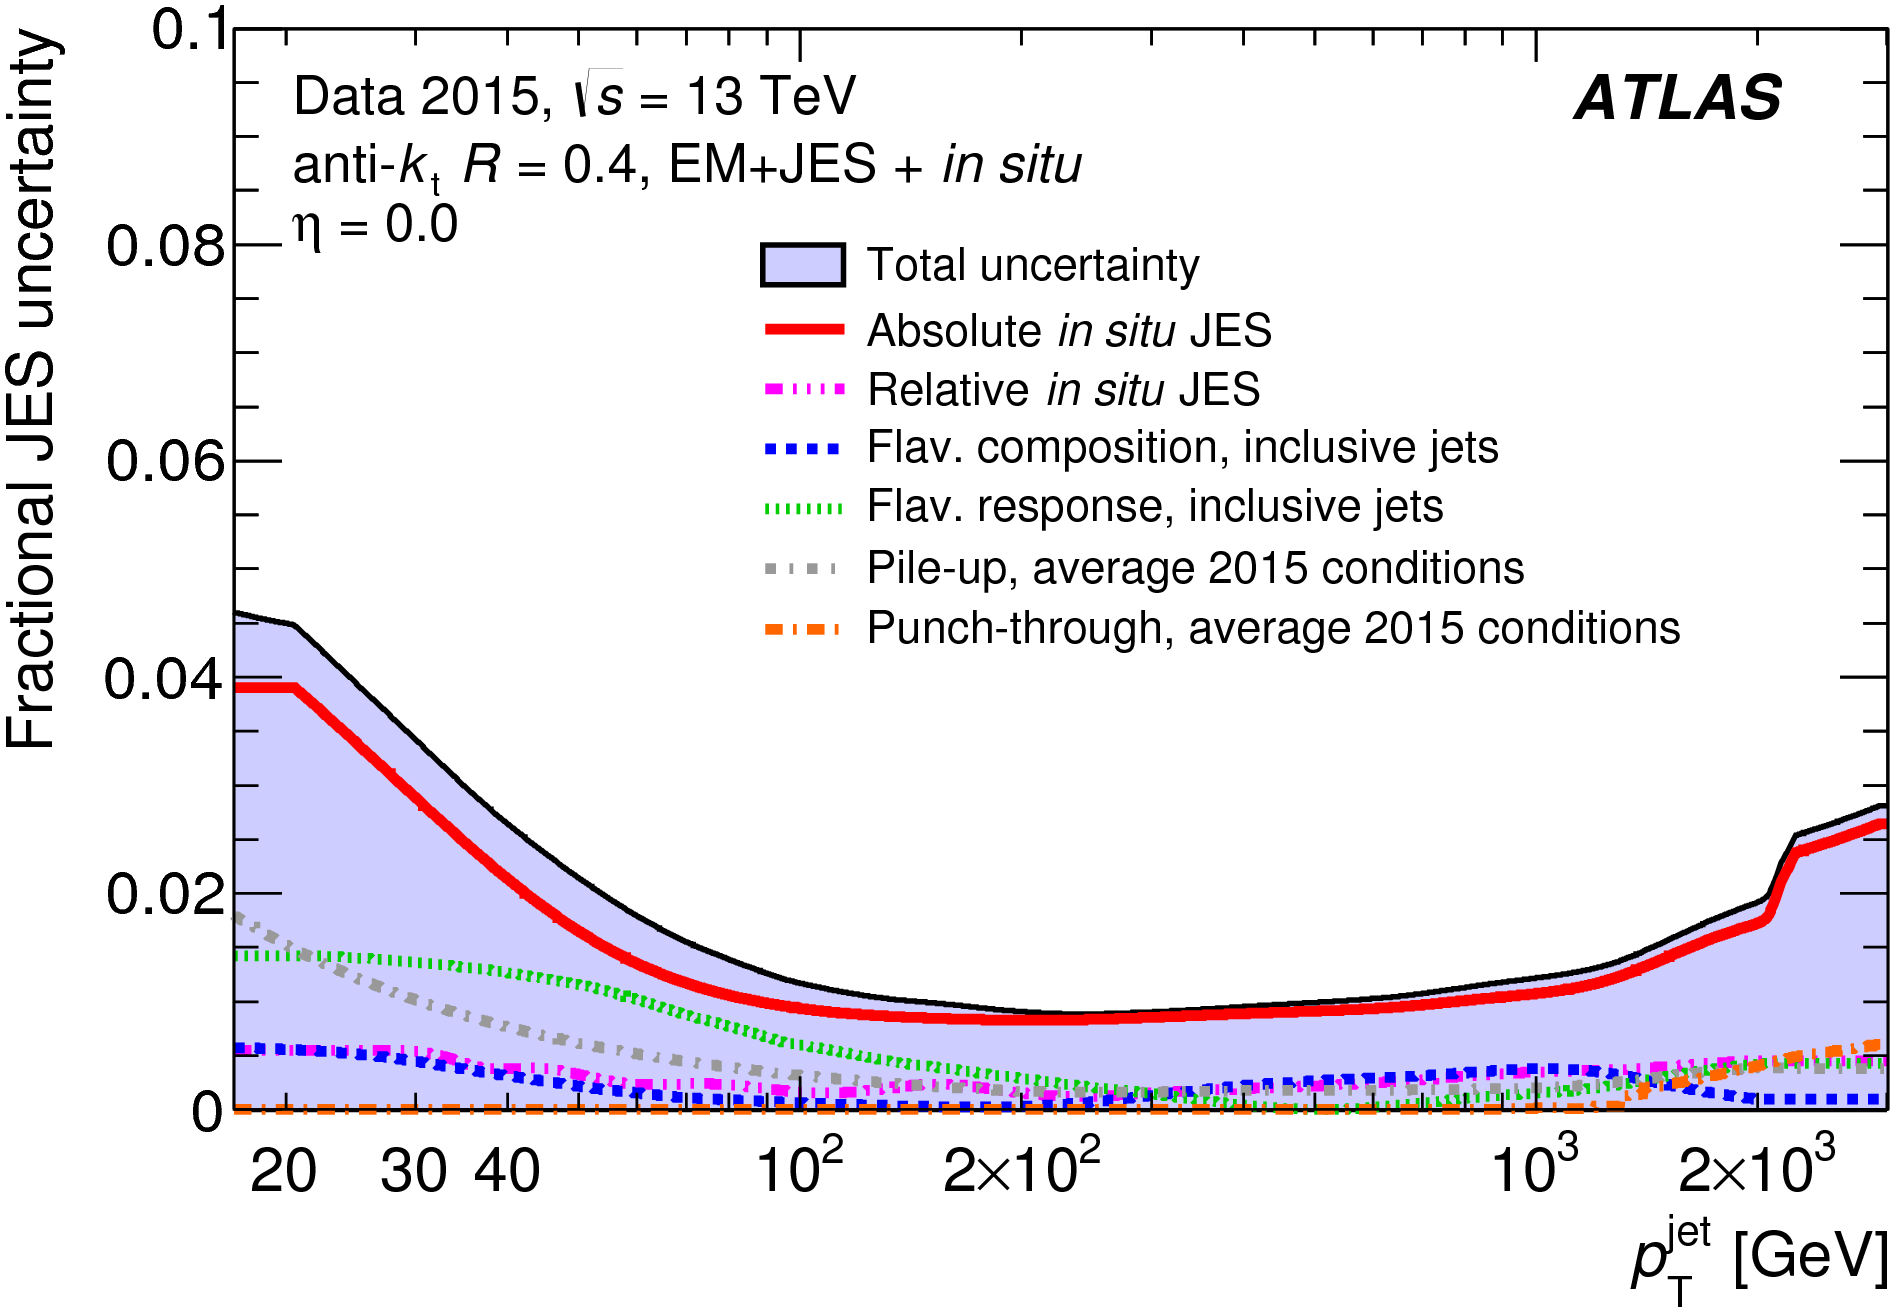
\includegraphics[width=0.7\columnwidth]{figures/Results/JES_Uncertainty.png}
%	\caption{Combined uncertainty in the JES of fully calibrated jets as a function of jet \pt at $\eta=0$.  Systematic uncertainty components include pileup, punch-through, and uncertainties propagated from $Z/\gamma$-jet and mulijet balance, as well as the $\eta$-intercalibration.  The flavor composition and response uncertainties assume a quark and gluon composition taken from Pythia dijet MC simulation (inclusive jets).}
%	\label{fig:JES_Uncertainty}
%\end{figure}
%
%\subsection{Luminosity Uncertainty}
%A luminosity uncertainty is applied as a scale factor to the normalization of the various signal samples used in the resonance analysis.  For the combined 2015+2016 dataset, the uncertainty on the luminosity is 3.2\%.  This value was derived from a preliminary calibration of the luminosity scale using the results of the two van der Meer scans performed in August 2015 and May 2016.  In these scans, the x-y beam separation of the two low intensity beams is scanned over, allowing for a measurement of the visible cross-section.  The method used is similar to the Run-1 method documented in~\cite{Luminosity}.
%
%\subsection{Function Choice Uncertainty}
%To estimate an uncertainty in the choice of fit function, an additional sliding window fit was performed using Eq.~\ref{eq:dijet} with $p_4\neq0$.  The result of the fit is compared to the result of the nominal three-parameter fit, and the average difference between the two fit results across a set of pseudodata drawn from Poisson fluctuations of the nominal background fit is taken as an uncertainty.  The fit uncertainty is shown by the light blue line in Figure~\ref{fig:FitUncertainty}; the uncertainty is only in one direction unlike most other sources of uncertainty.
%
%\subsection{Statistical Uncertainty}
%
%The statistical uncertainty in the fit is calculated in a similar method to the function choice uncertainty, using pseudodata drawn from the nominal fit to data.  The uncertainty in each $m_{jj}$ bin is taken to be the root mean square of the fit results for that bin across all pseudo-experiments.  The statistical uncertainty is shown by the dark blue line in Figure~\ref{fig:FitUncertainty}.
%
%\begin{figure}[ht!]
%	\centering
%	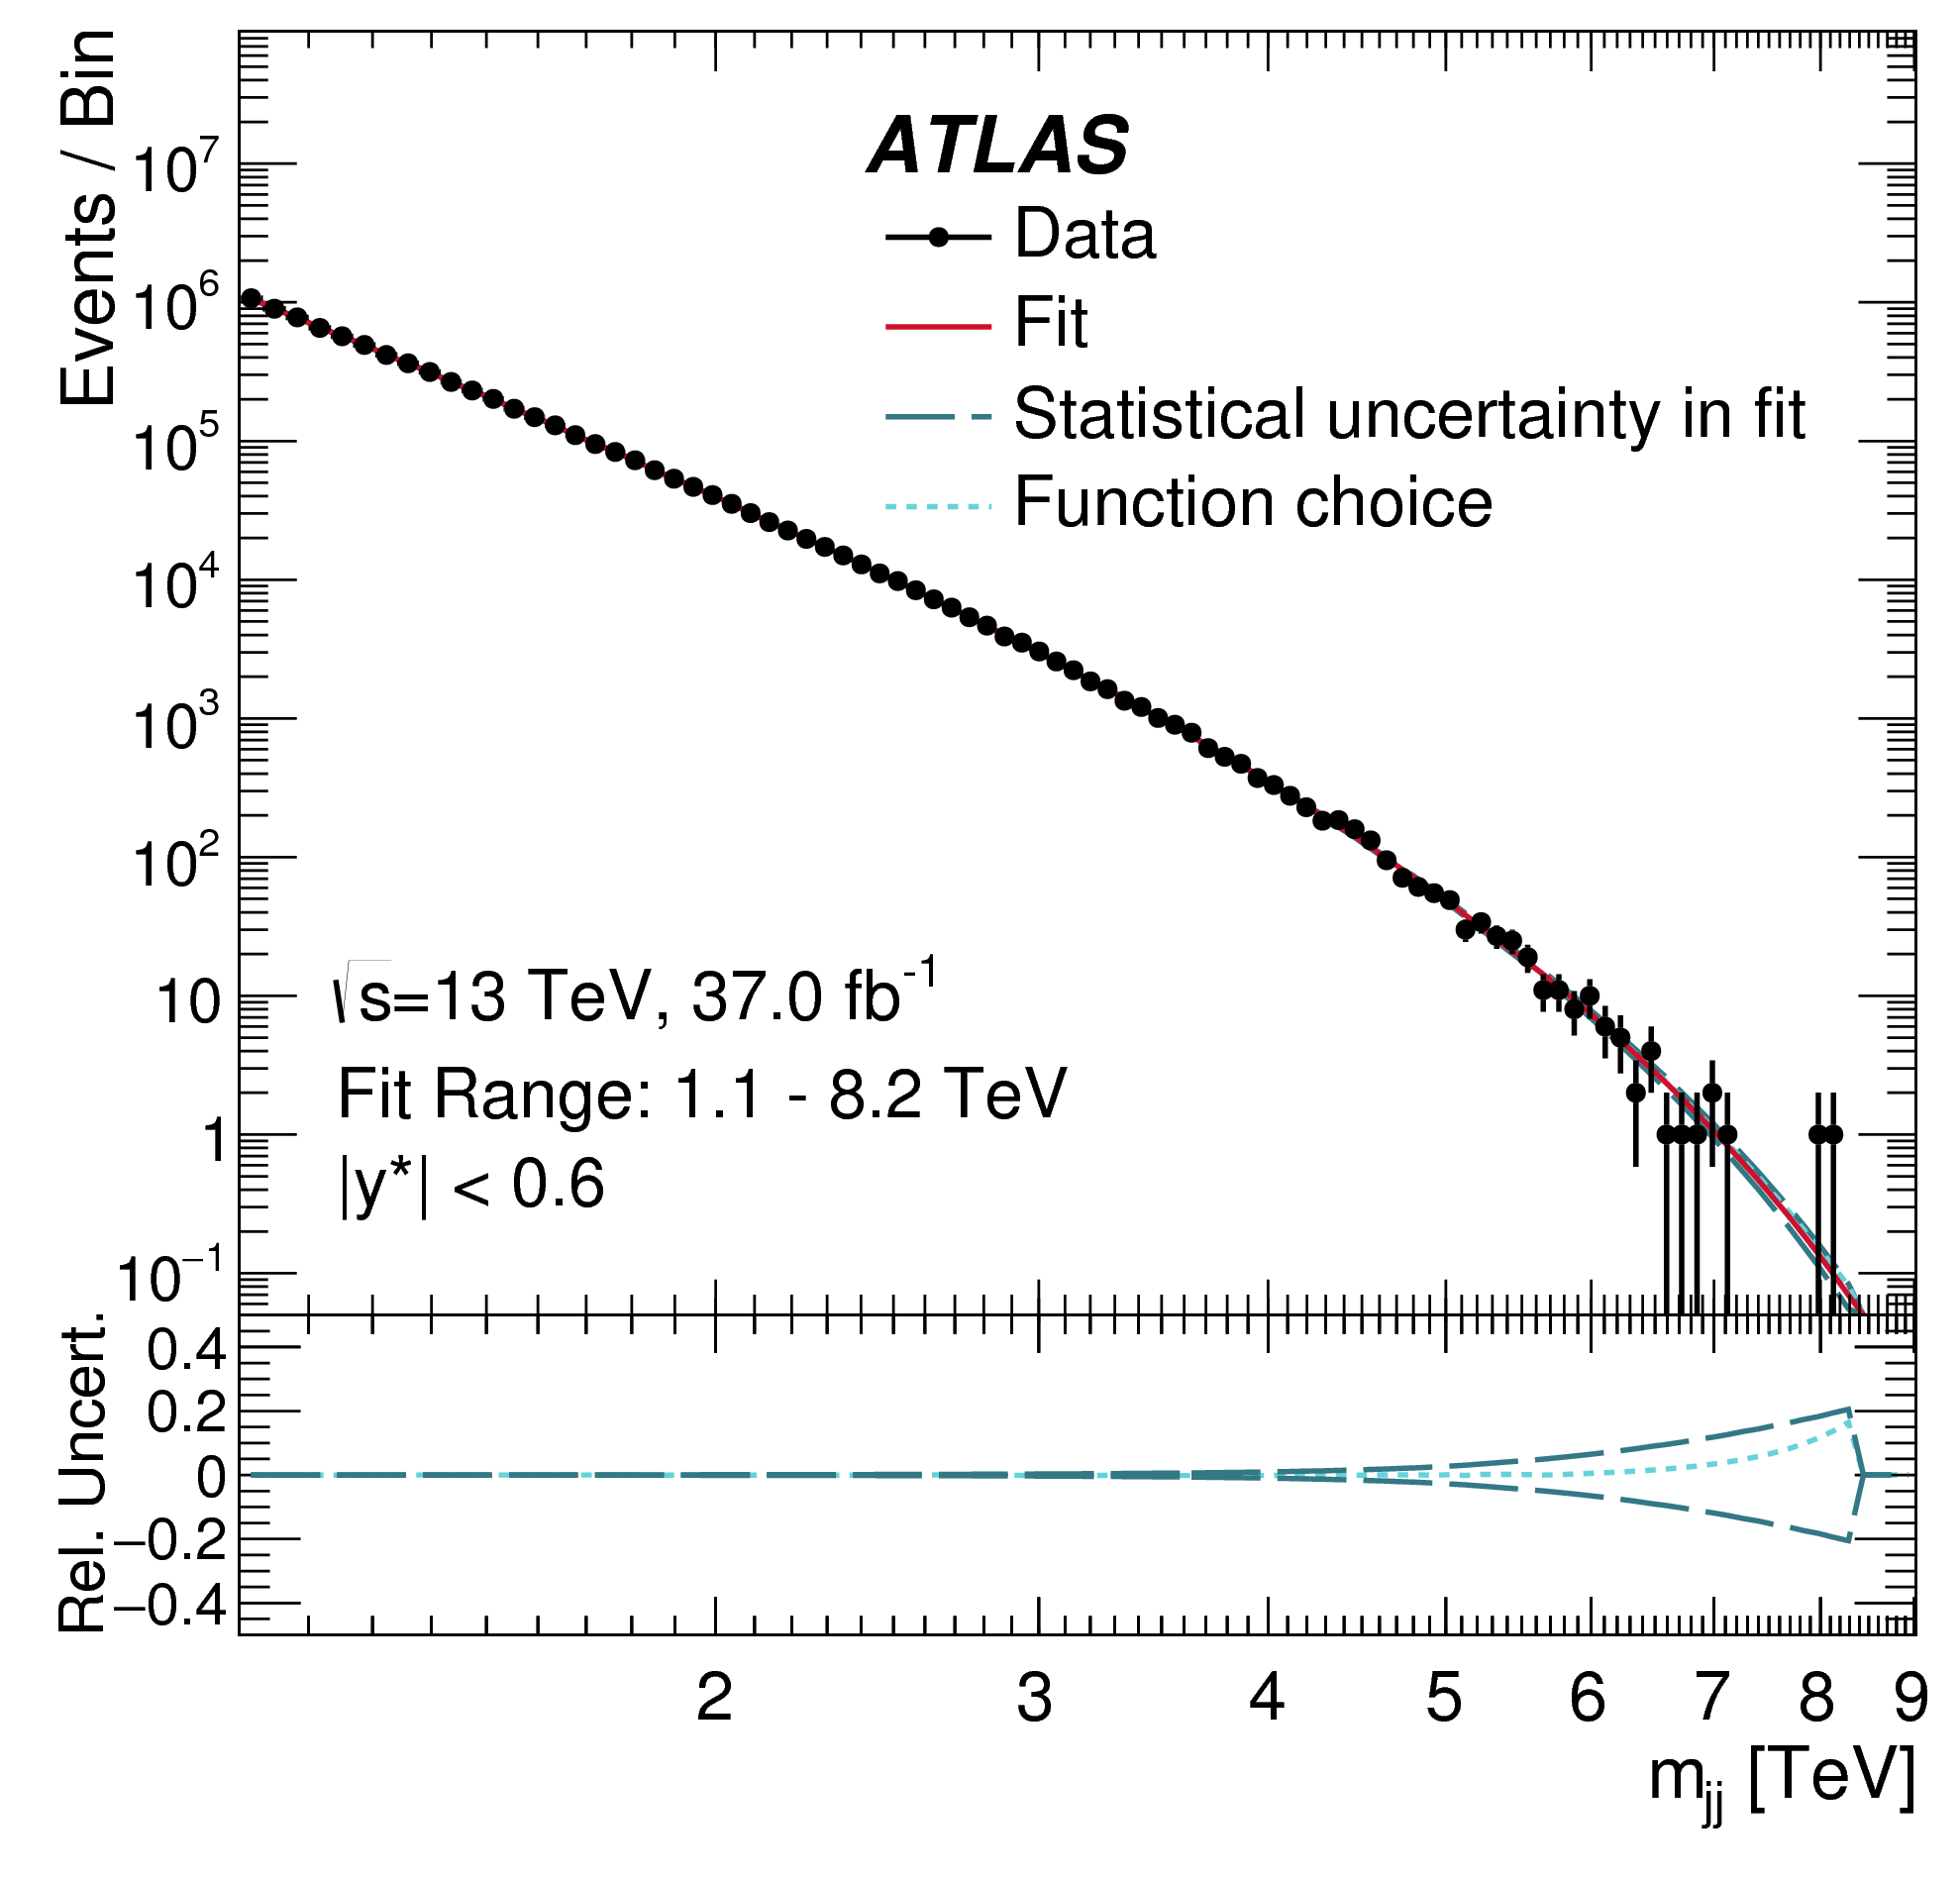
\includegraphics[width=0.5\columnwidth]{figures/Results/FitUncertainty.png}
%	\caption{The sliding window fit to the $m_{jj}$ distribution with $|y^*|<0.6$~(red) with its two uncertainties. The dark blue line with long dashes indicates the statistical uncertainty in the fit, corresponding to the variability in the fit results across a large collection of pseudoexperiments. The light blue line with short dashes indicates the uncertainty in the function choice, based on comparison to a function with a higher number of parameters. Statistical uncertainty is shown at the one-sigma level, while the function uncertainty shown is the mean difference between the nominal and alternate functions.}
%	\label{fig:FitUncertainty}
%\end{figure}
%
%\section{Limits on Benchmark Signals}
%
%Starting from the invariant mass distribution obtained from the search selections, the previously descibed Bayesian method is applied to the data and simulated signal samples to set 95\% credibility-level (CL) upper limits on the cross-section times acceptance.  The limit is interpolated between the discrete simulated mass points to create a continuous exclusion curve.
%
%Figure~\ref{fig:Limits} shows the observed and expected limits for the benchmark signals with the data shown as black points and the theory curve in dashed blue.  Limits are set on the product of cross-section times acceptance times branching ratio ($\sigma \times A \times$ BR); the efficiency for all signal models is approximately 1.  Expected limits are shown by the black dashed line, and the 1$\sigma$ and 2$\sigma$ bands which describe the sensitivity of the analysis to random fluctuations of the data are denoted by the yellow and green curves.  The observed data points are the black points, and the theory curve for each benchmark model is shown in blue.  No uncertainties are assessed for the theoretical cross-sections.
%
%\begin{figure}[ht!]
%	\centering
%	\subfloat[]{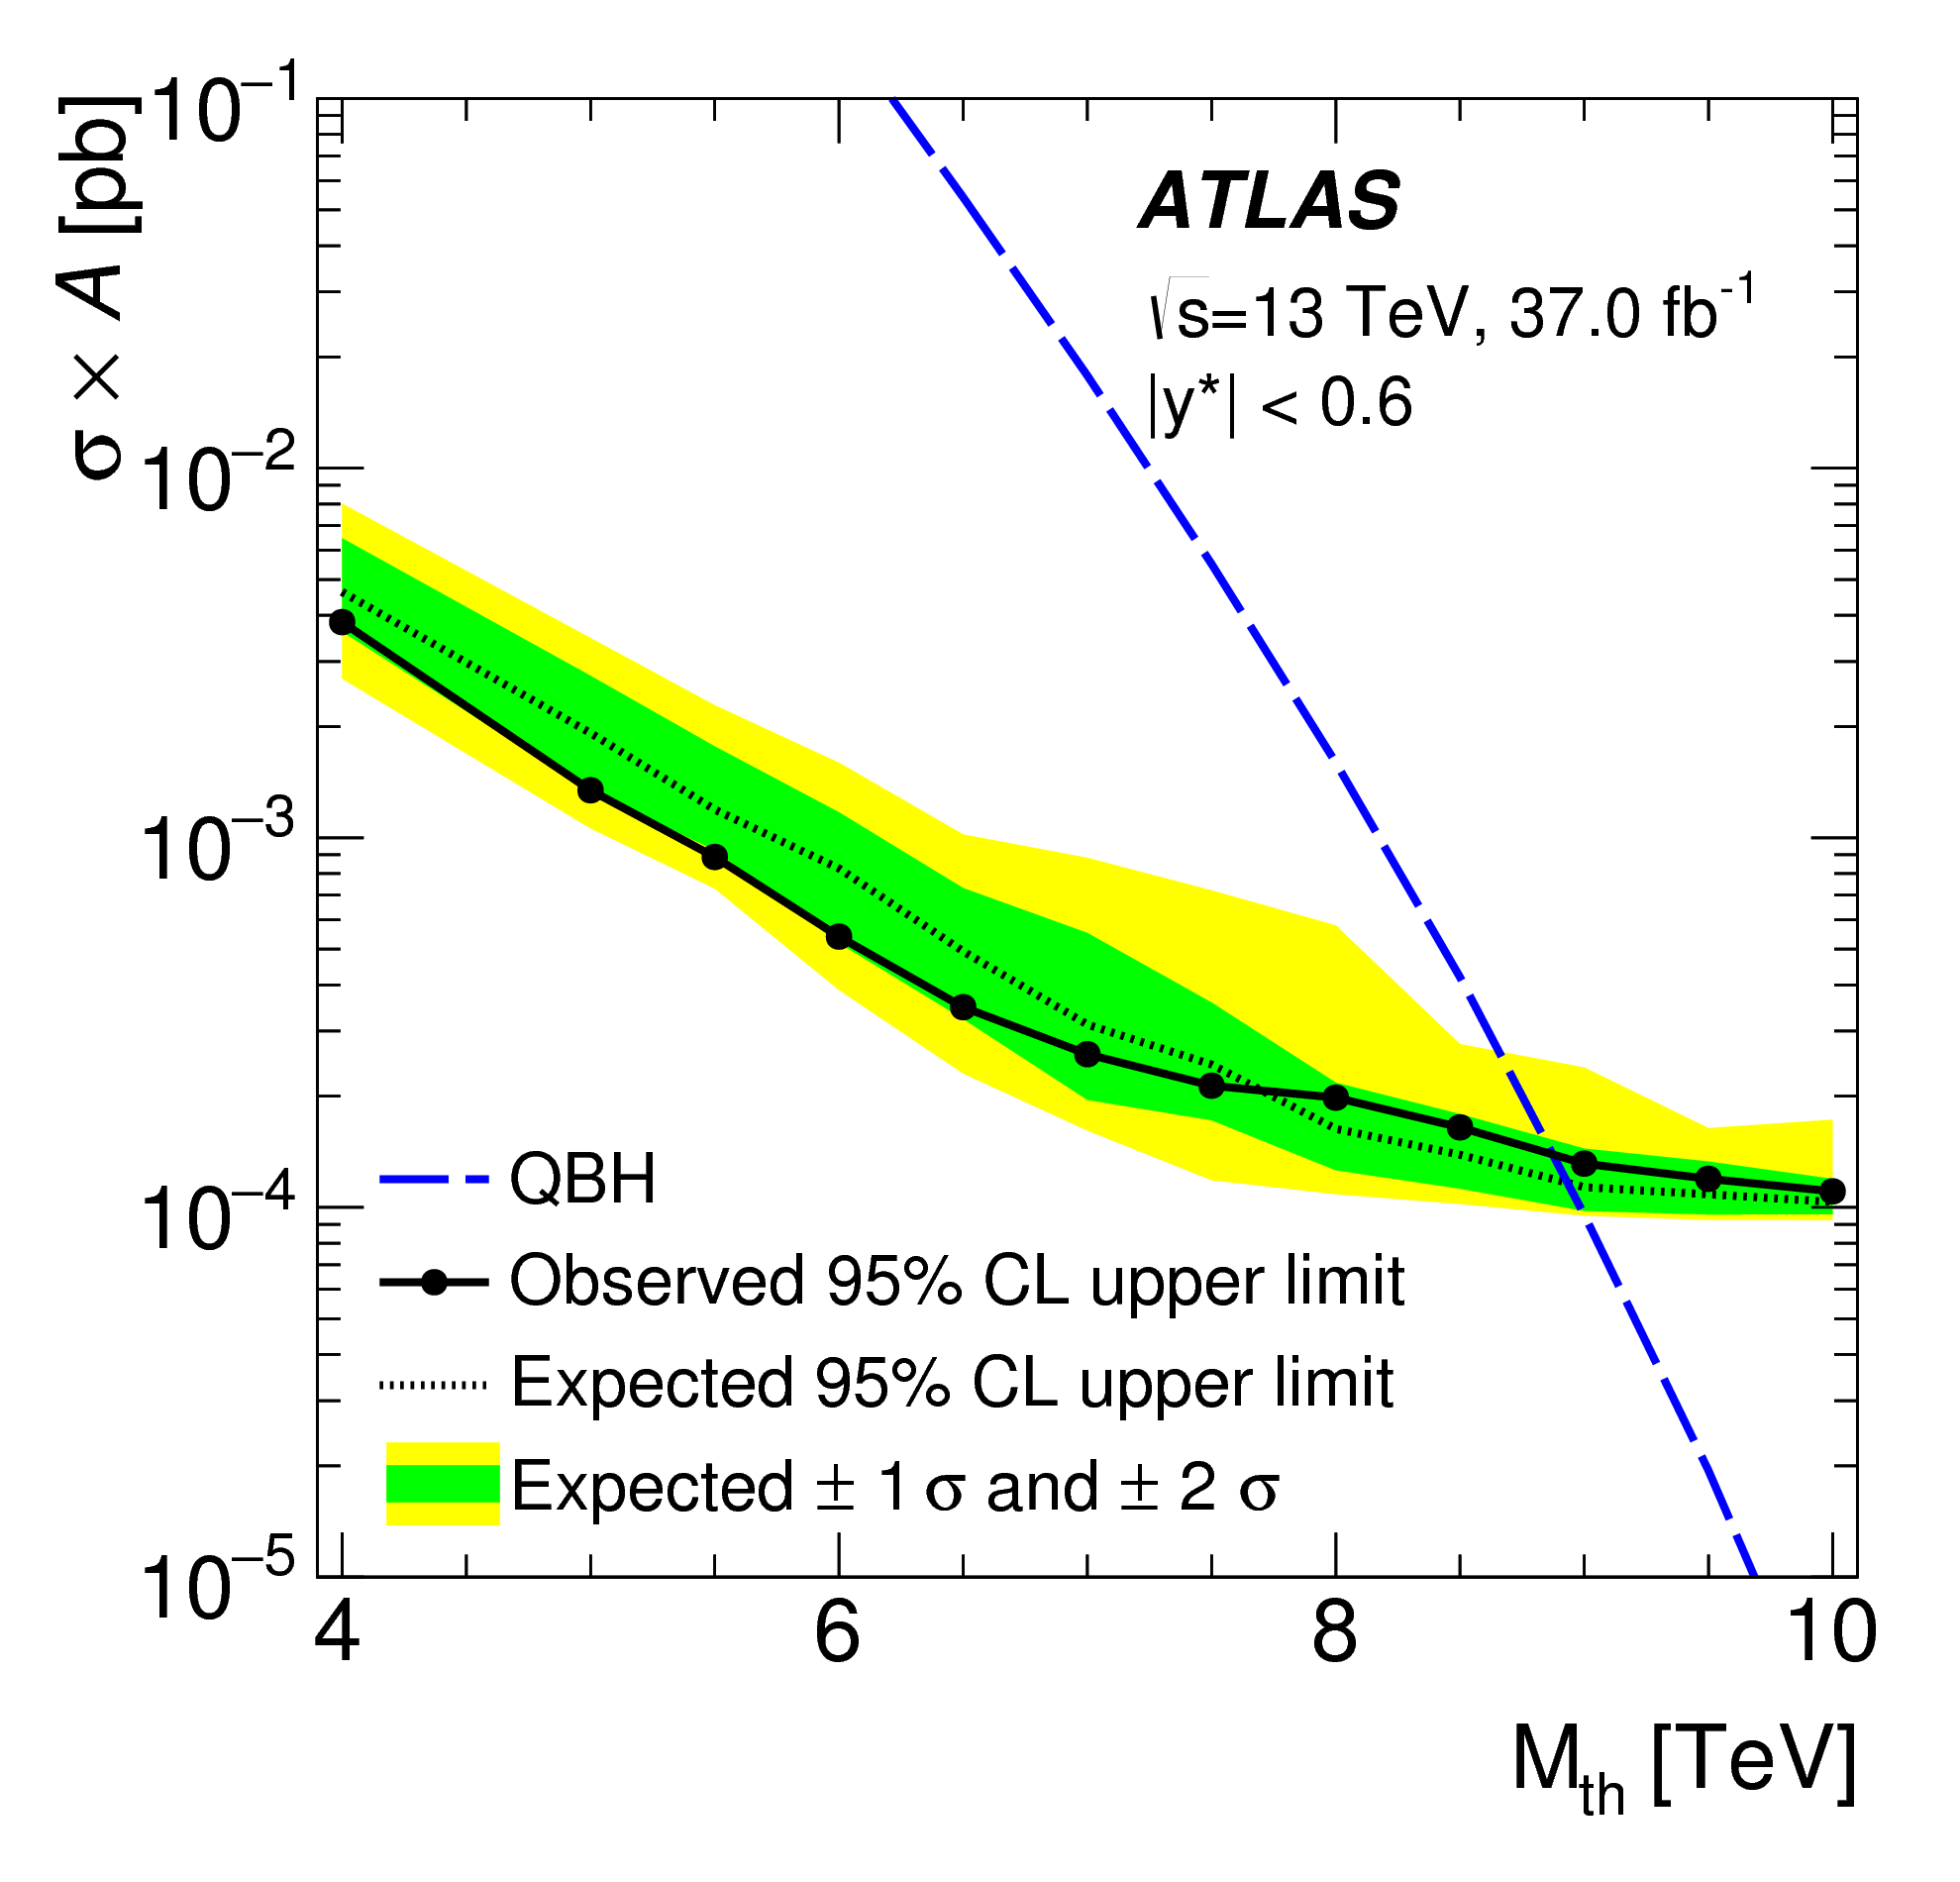
\includegraphics[width=0.45\columnwidth]{figures/Results/QBHLimit.png}\label{subfig:QBHLimit}}
%	\hspace{0.1\columnwidth}%
%	\subfloat[]{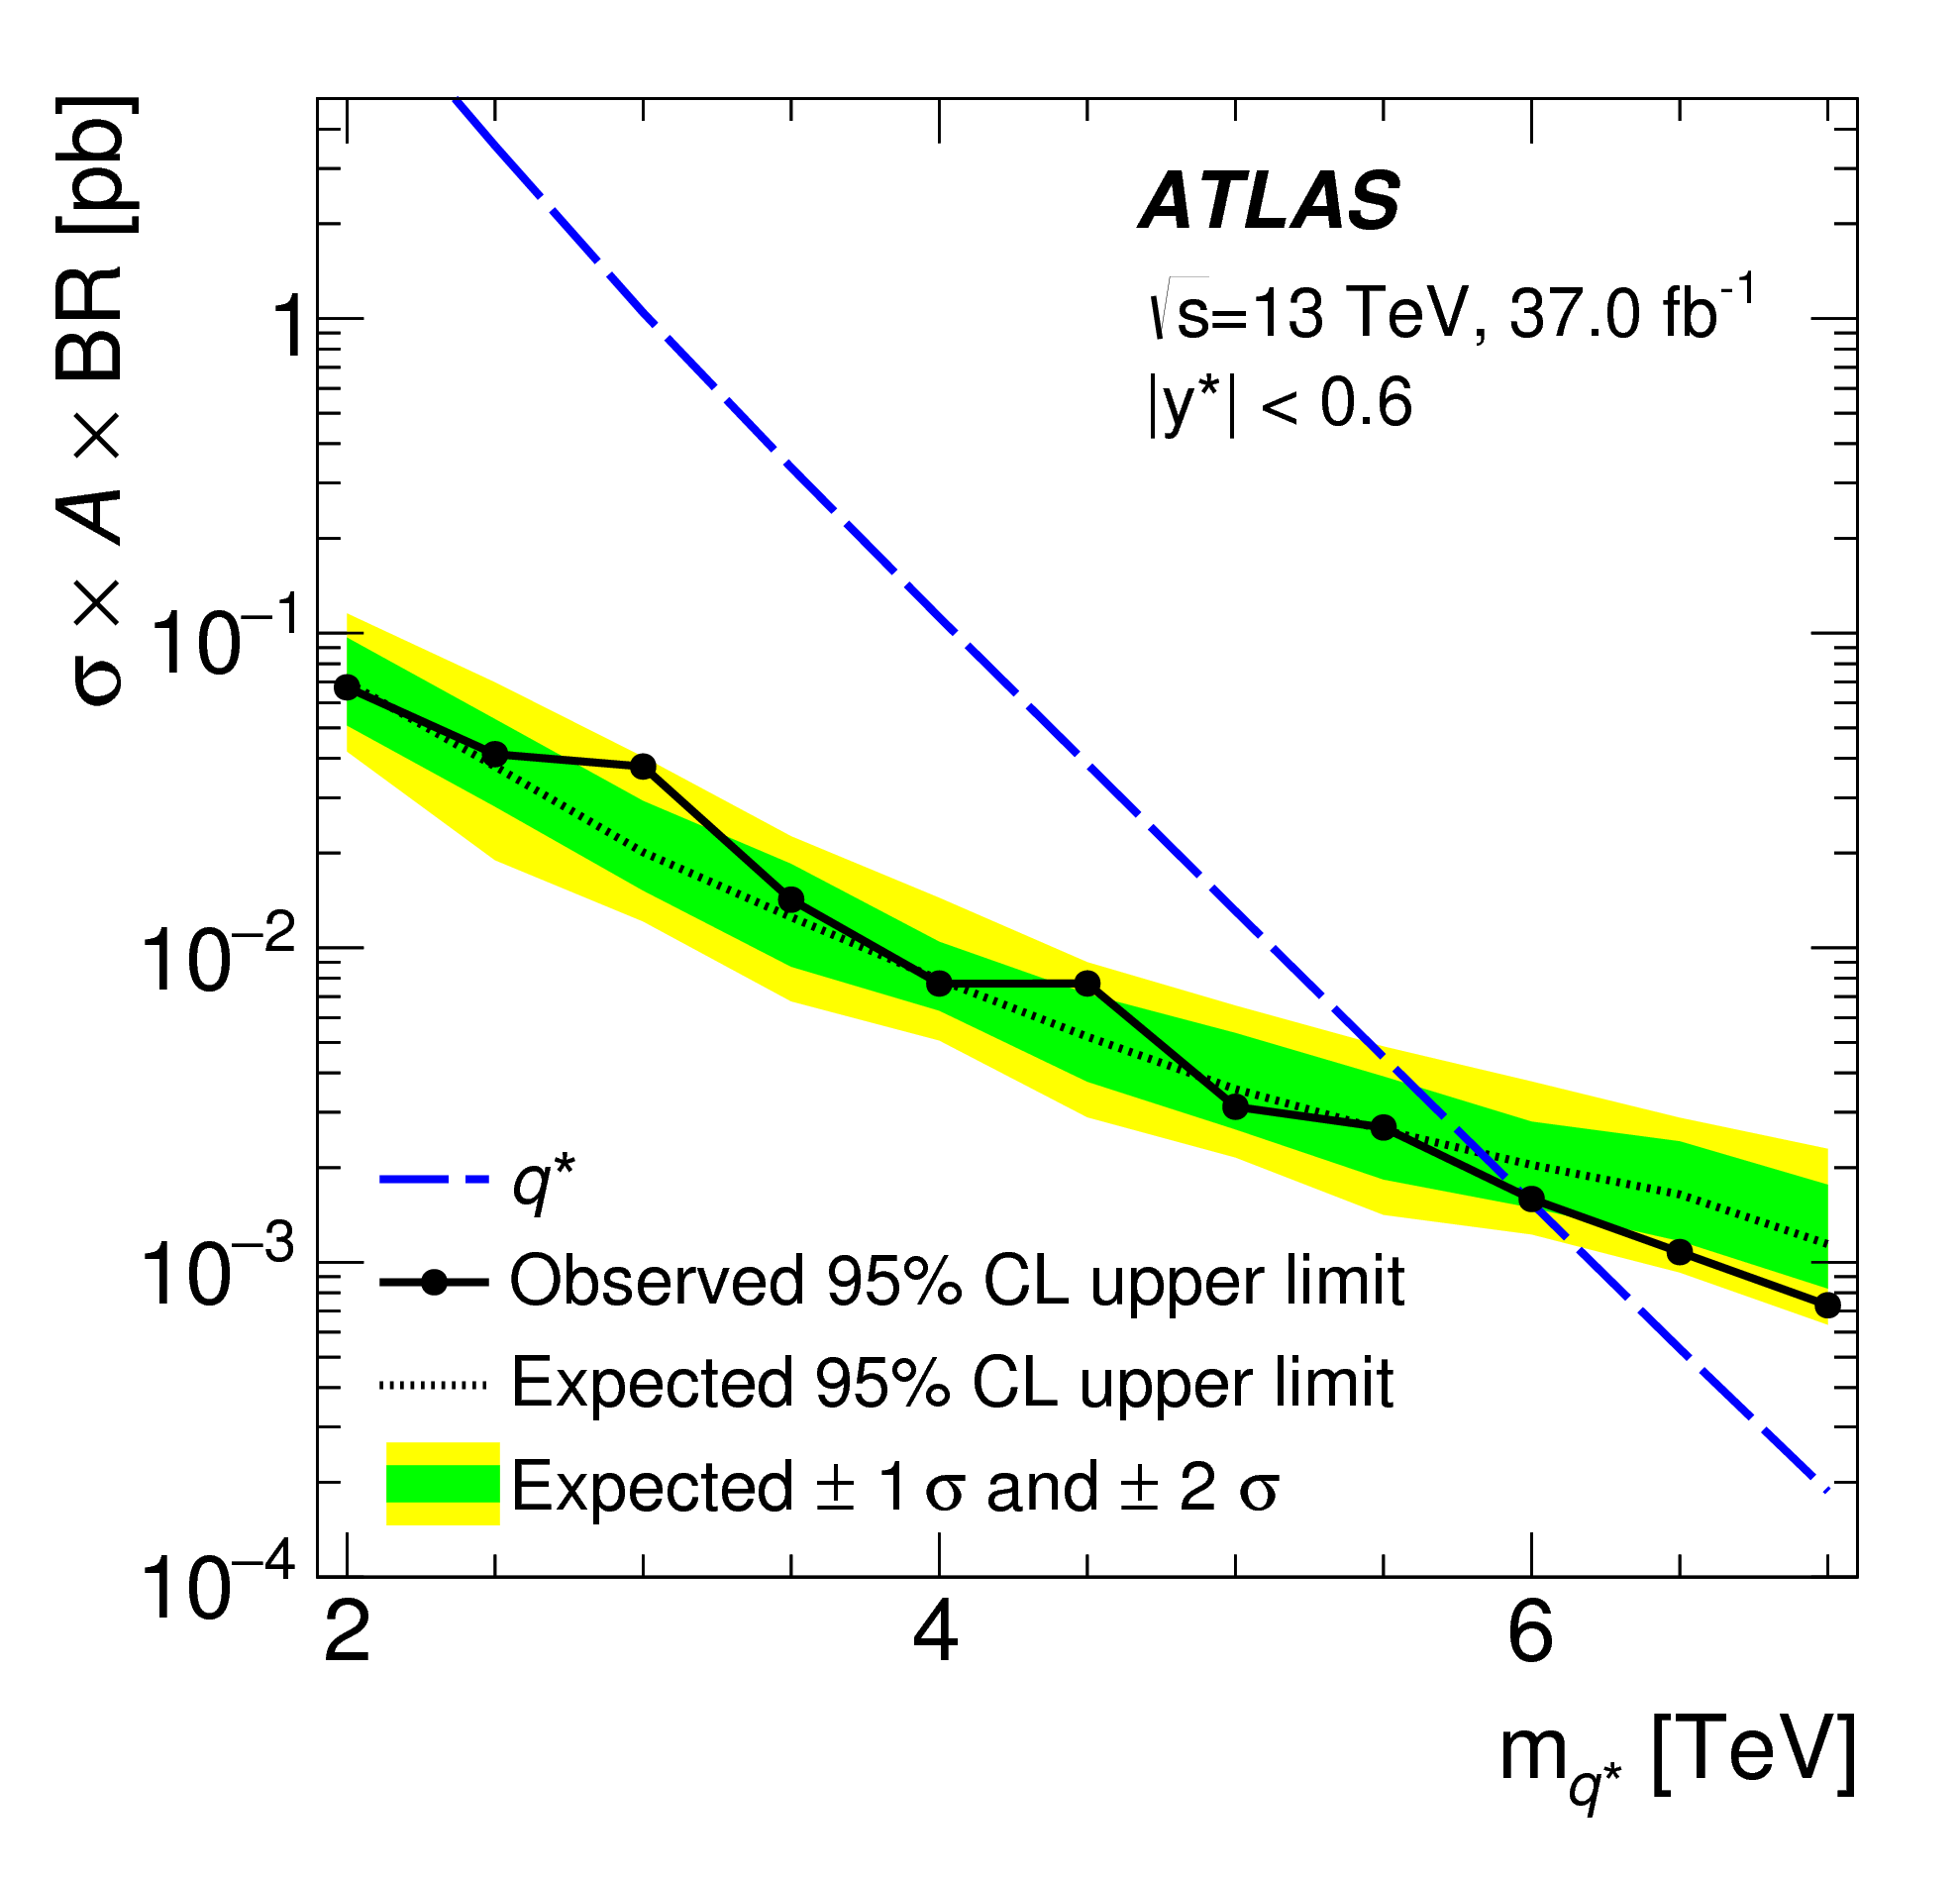
\includegraphics[width=0.45\columnwidth]{figures/Results/QStarLimit.png}\label{subfig:QStarLimit}}
%	\hspace{0.1\columnwidth}%
%	\subfloat[]{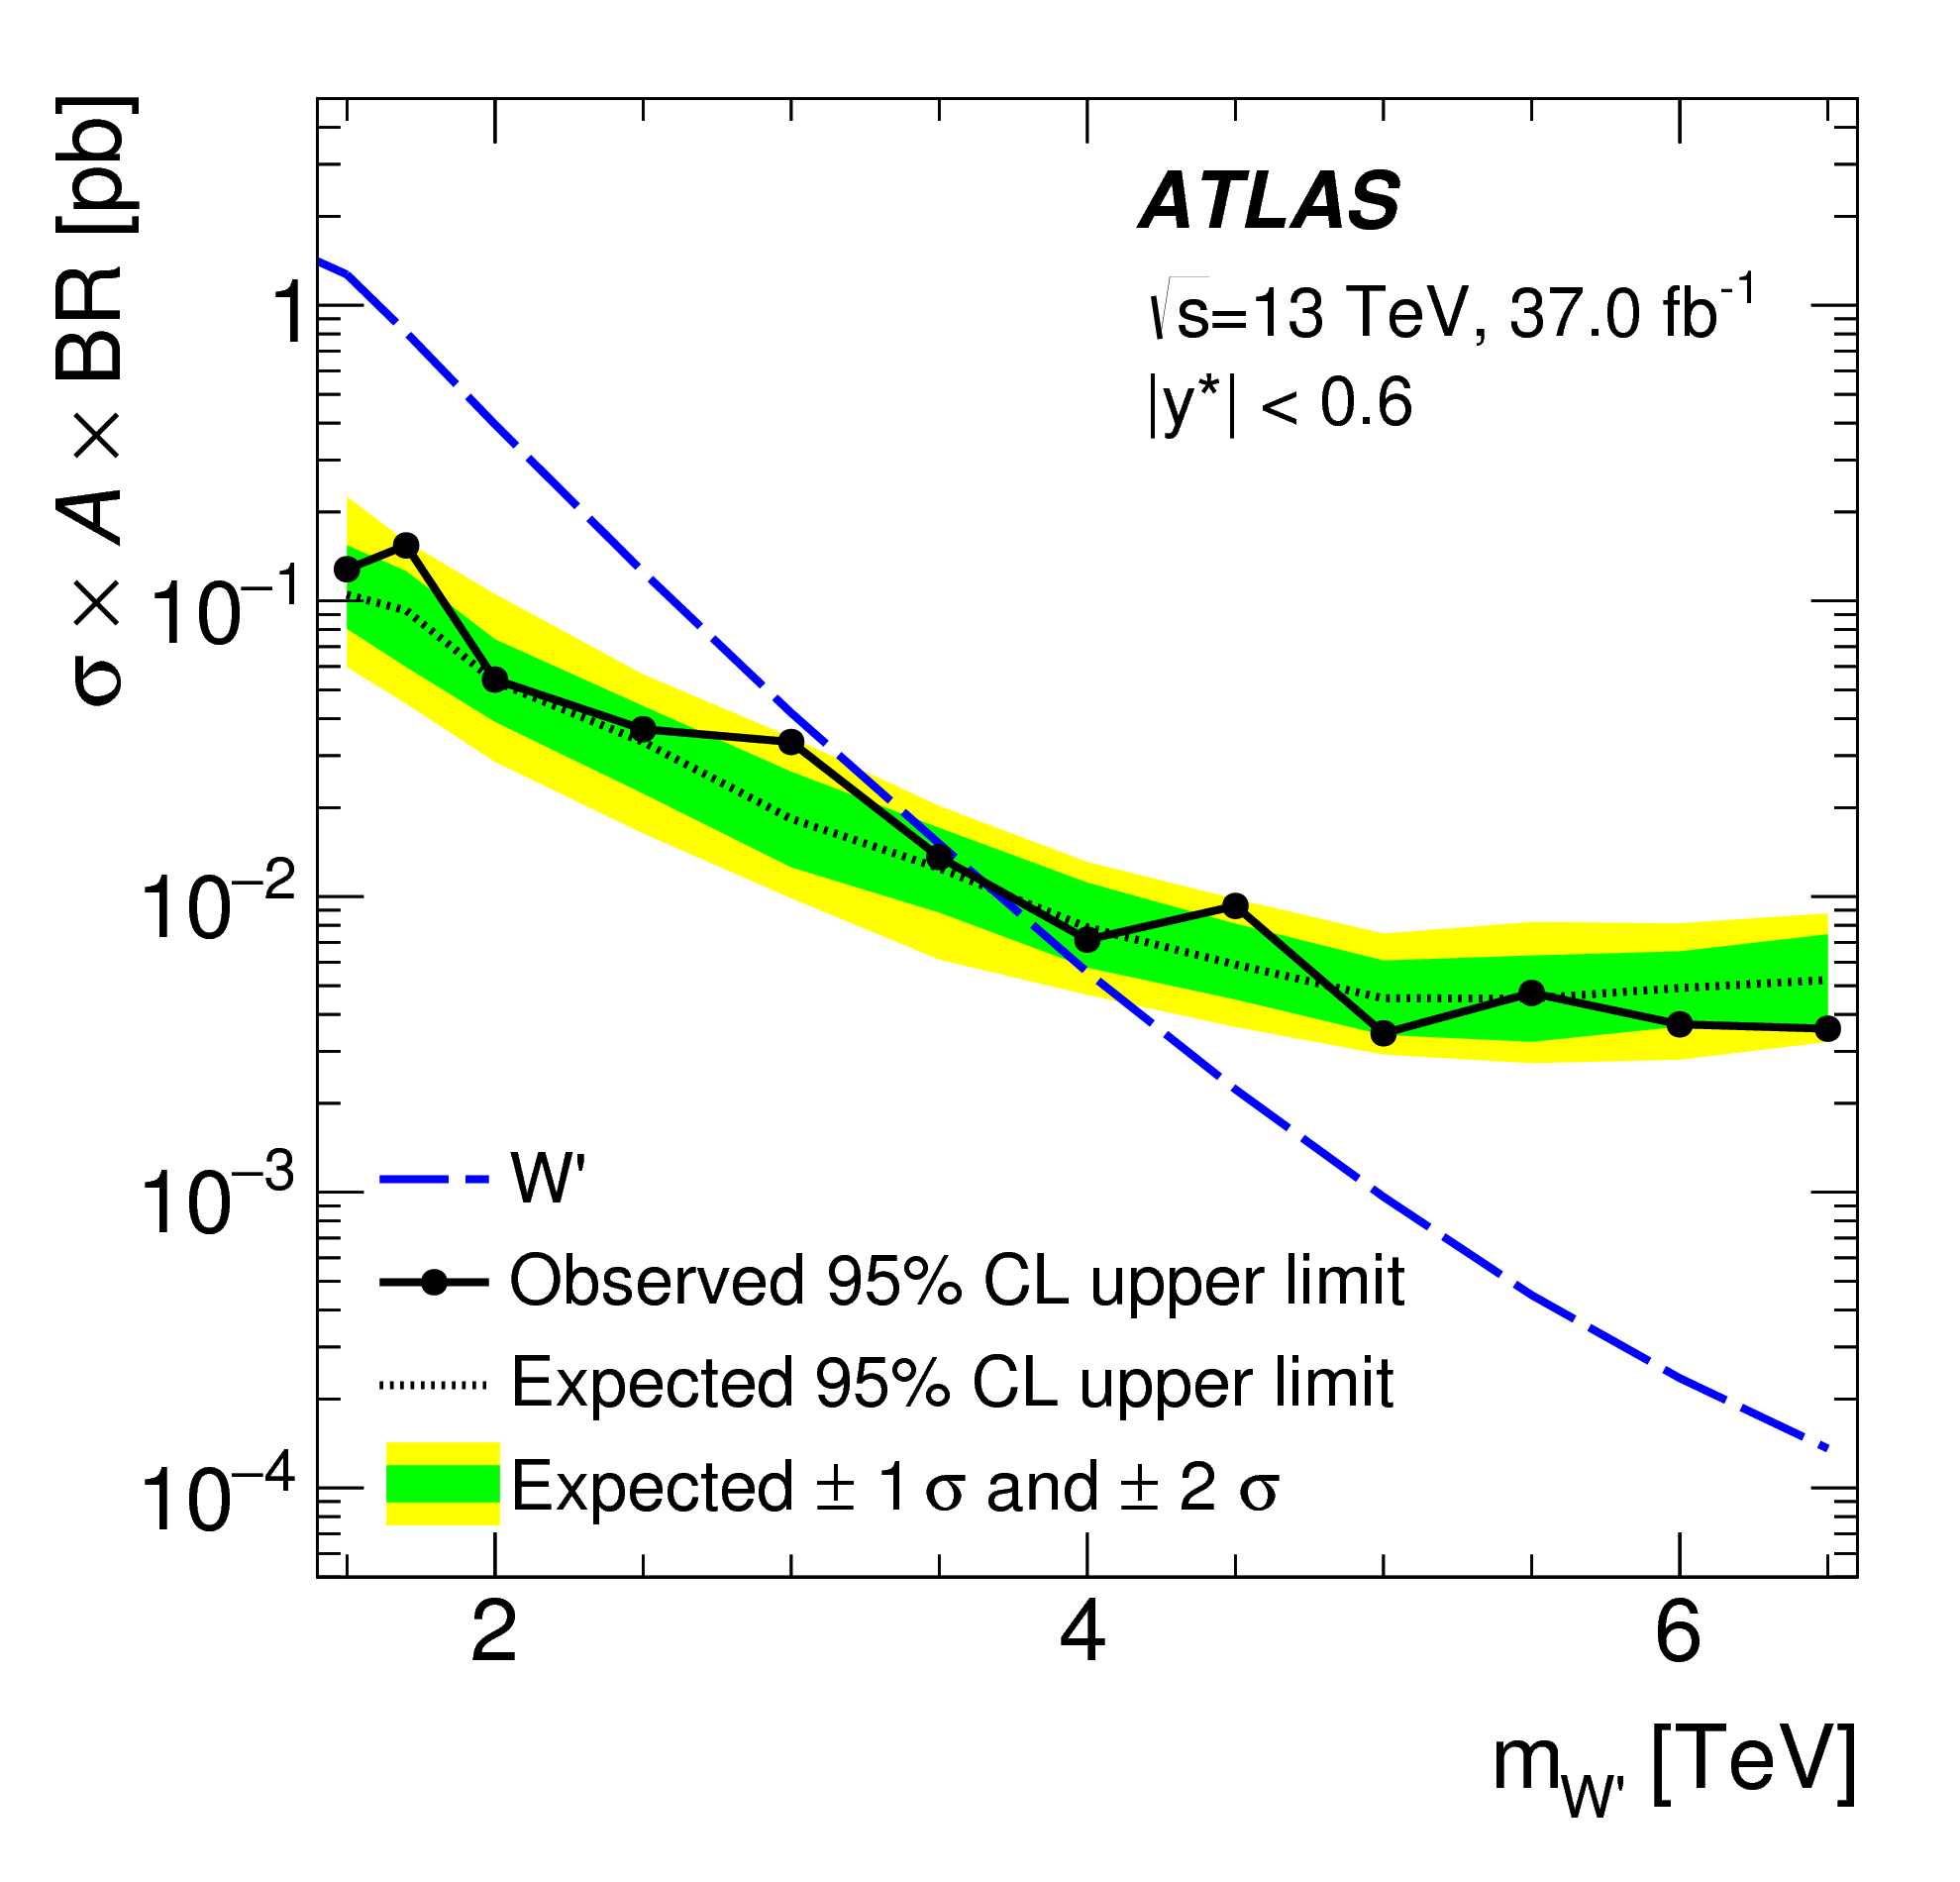
\includegraphics[width=0.45\columnwidth]{figures/Results/WPrimeLimit.png}\label{subfig:WPrimeLimit}}
%	\hspace{0.1\columnwidth}%
%	\subfloat[]{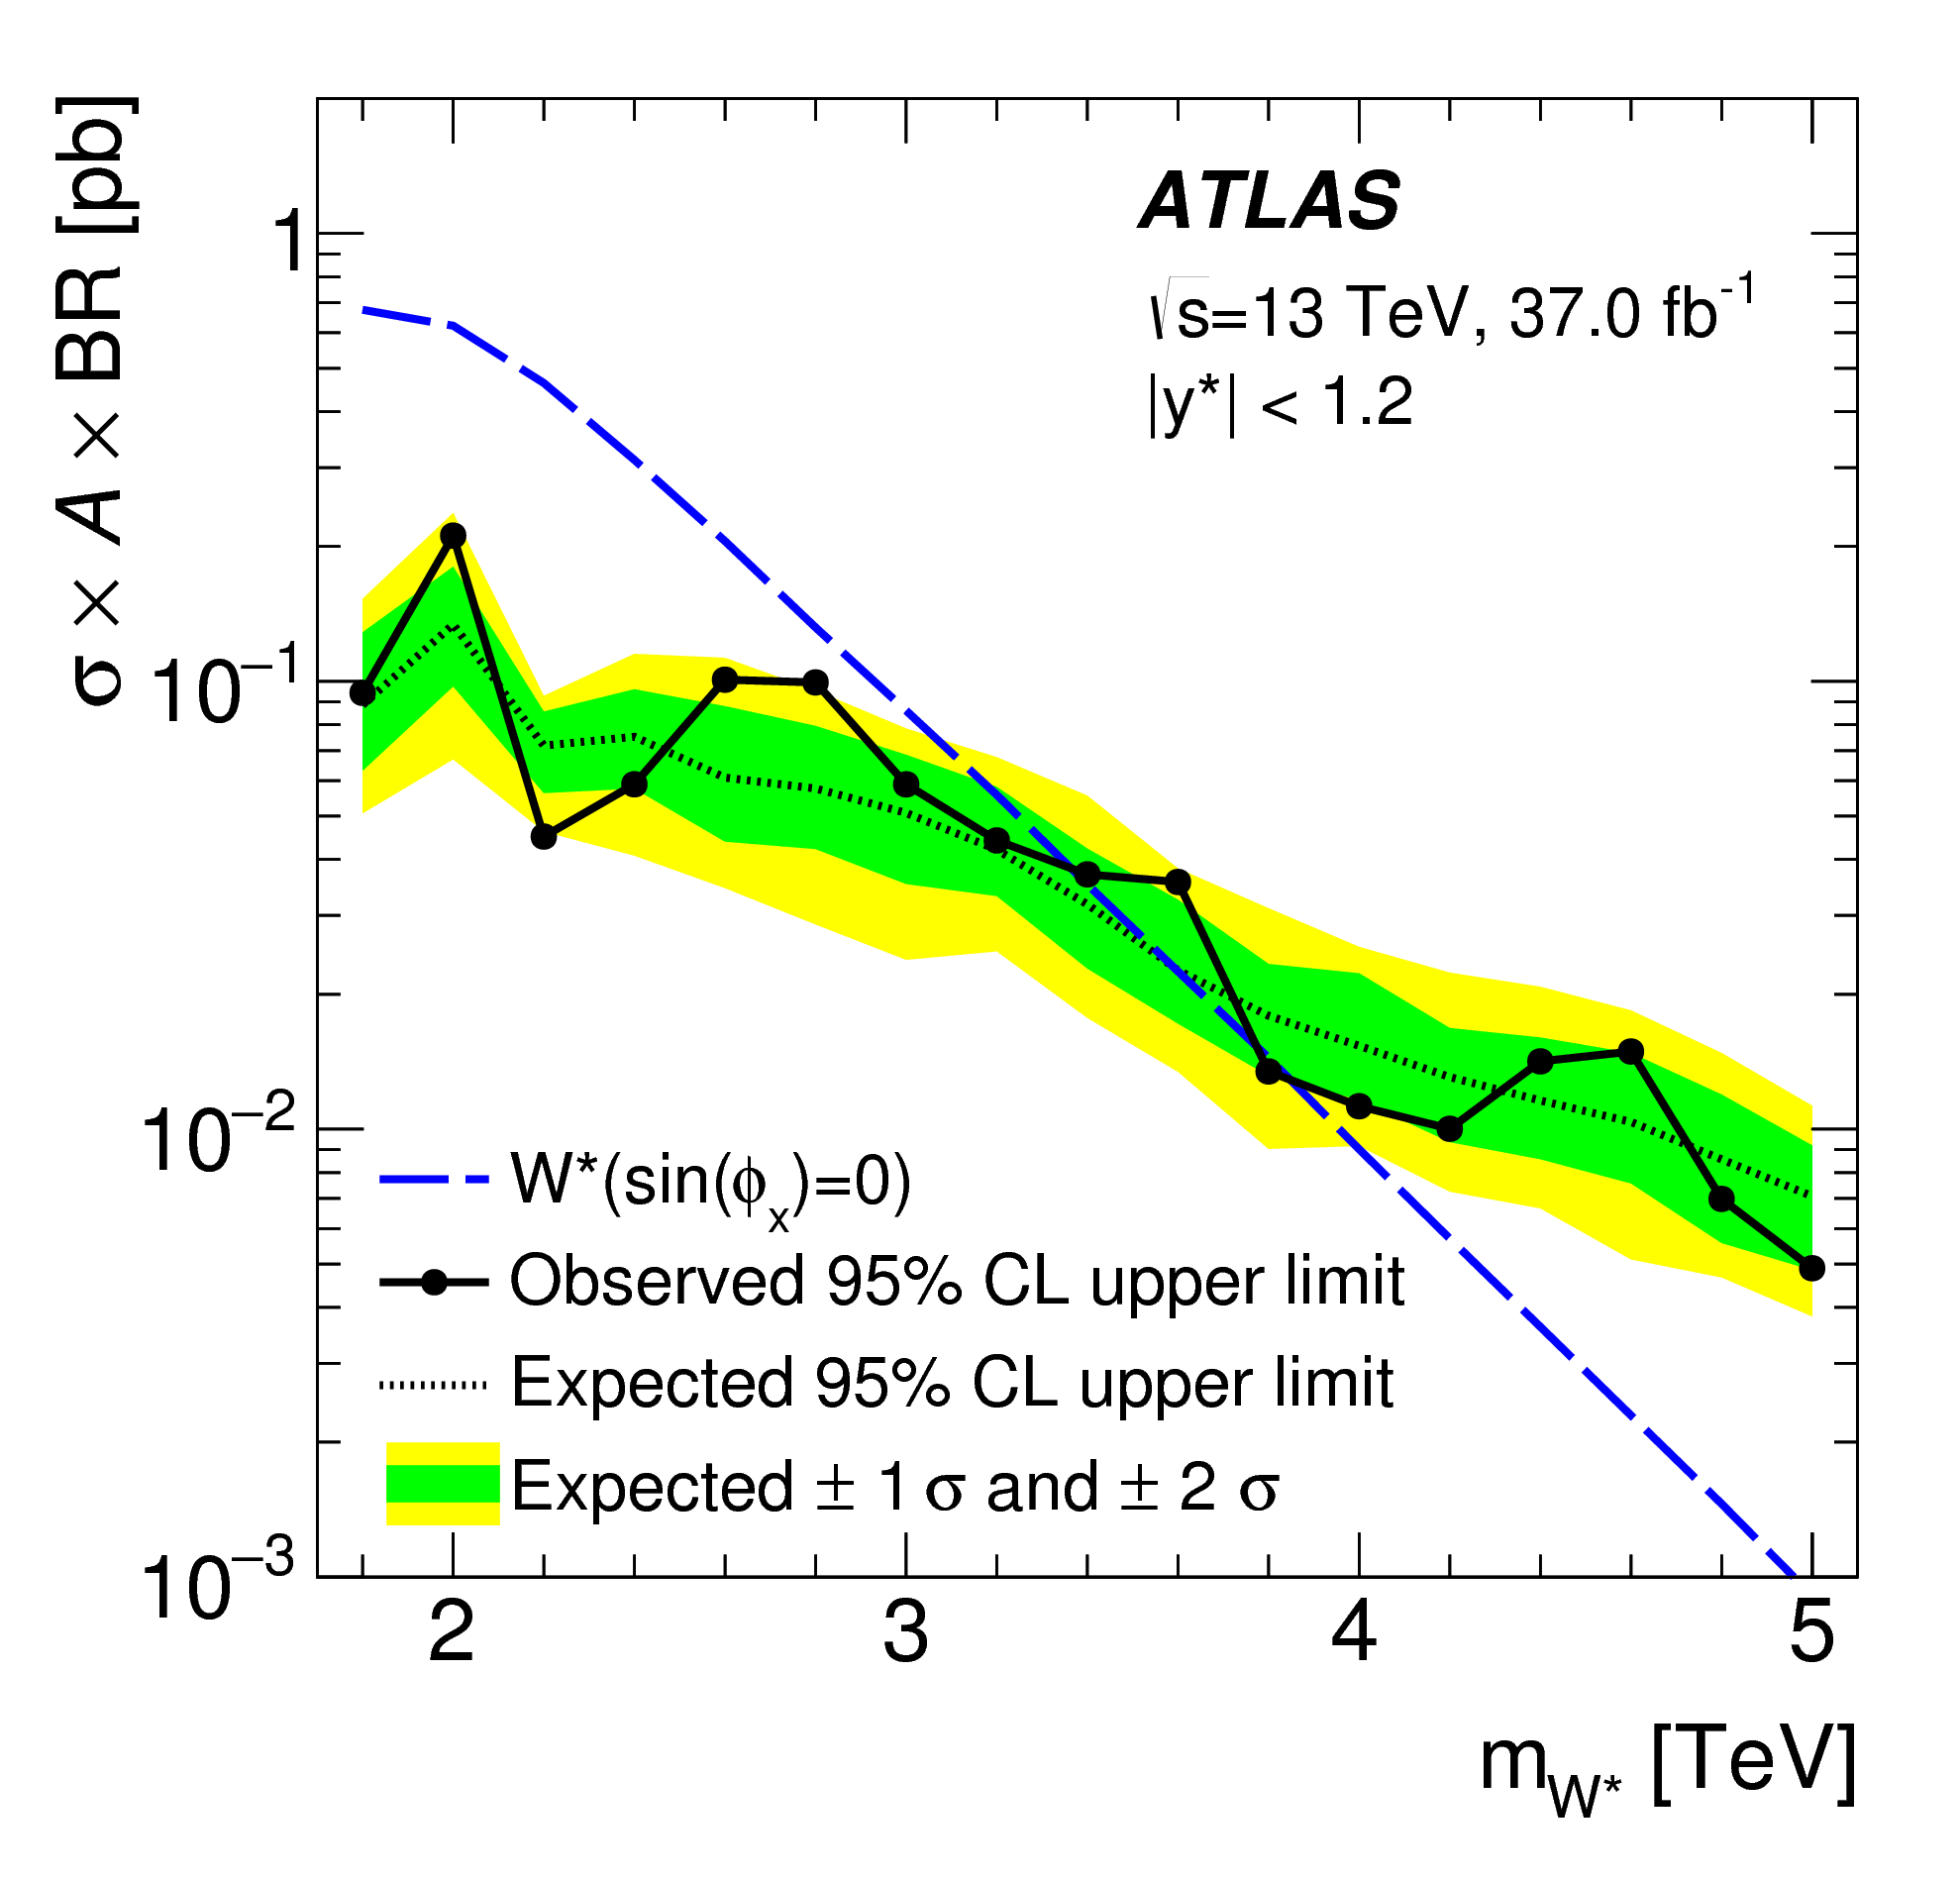
\includegraphics[width=0.45\columnwidth]{figures/Results/WStarLimit.png}\label{subfig:WStarLimit}}
%	\caption{Limits on the cross-section times branching ratio times acceptance for the three resonance benchmark models (a) Quantum black holes (ADD, n=6 model) (b) excited quarks (c) $W'$ bosons, and (d) $W^*$ bosons.  The first three limits use the nominal selection while the fourth uses the widened $y^* < 1.2$ selection.  The theory cross-section is given by the blue dashed line.}
%	\label{fig:Limits}
%\end{figure}
%
%This analysis sets observed (expected) 95\% CL exclusion limits on these benchmarks: 6.0 (5.8)\,TeV for excited quarks, 3.6 (3.7)\,TeV for $W'$ bosons, 3.4 (3.6)\,TeV for $W^*$ bosons, and 8.9 (8.9)\,TeV for quantum black holes.  These limits compare favorably to the limits obtained by CMS using an equivalent amount of data, as shown in Table~\ref{tab:LimitCompare}.
%
%
%\begin{table}[]
%	\centering
%	\begin{tabular}{l c c}
%		\toprule
%		\multicolumn{3}{c}{Observed (Expected) 95\% CL Exclusion Limits} \\
%		\midrule
%		Benchmark Model & ATLAS (37\,\ifb) & CMS (36\,\ifb)  \\
%		\midrule
%		Excited Quark & 6.0(5.8)\,TeV & 6.0(5.8)\,TeV\\
%		\midrule
%		$W'$ & 3.6(3.7)\,TeV & 3.3(3.6)\,TeV \\
%		\bottomrule
%
%	\end{tabular}
%	\caption{Comparison of limits on benchmark models set by ATLAS~\cite{Dijet2017} and CMS~\cite{CMSDijet}.}
%	\label{tab:LimitCompare}
%\end{table} 
%
%Limits for the dark matter mediator $Z'$ model are shown in the 2D plane of the $Z'$ mass and the coupling to quarks, $g_q$.  Limits are set in the region between 1.5 and 3.5\,TeV, and all couplings above the curve (indicated by the hatching) are excluded up to $g_q=0.5$, as beyond that the resonance width grows beyond 15\% and becomes too wide to be properly detected by this analysis.  Signal points are simulated with spacing of 0.5\,TeV in mass and spacing between 0.05 and 0.1 in $g_q$; a smooth curve is created by interpolating between points in $g_q^2$ and $m_{Z'}$.
%
%\begin{figure}[]
%	\centering
%	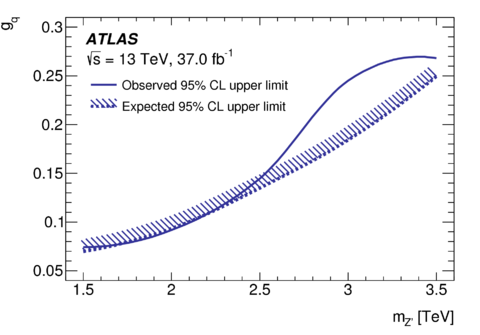
\includegraphics[width=0.8\columnwidth]{figures/Results/ZPrimeLimit.png}
%	\caption{95\% CL limits on the production of leptophobic $Z'$, shown in the 2D plane of the mass of the $Z'$ ($m_Z$) and the coupling to quarks ($g_q$).  The excluded region is the region in the plane above the solid line, as indicated by the hatching.  Exclusions are valid only up to $g_q=0.5$, as coupling values above that create resonances which are too wide to be properly detected by this search.}
%	\label{fig:ZLimits}
%\end{figure}
%
%Limits are also set on generic Gaussian signals, meant as a tool for the theory community to help interpret the results by providing a point of comparison for any signal model with an approximately-Gaussian peak in the dijet invariant mass distribution.  The Gaussians used are trimmed to the central 95\% of events to eliminate long tails, and limits are set on varying widths from 0\% to 15\%.  The ATLAS results are given at particle level; this is achieved by creating a Monte Carlo-based transfer matrix which relates the particle level and reconstructed observables.  This allows for limits to be set on a given signal model, in this case a Gaussian shape, without the need for any additional information about the detector response.  For sufficiently narrow resonances, these results can be used to set limits on other BSM models by comparing them to a signal shape at particle level after applying the event selection used in this analysis.  The limits on Gaussian signal shapes are shown in Figure~\ref{fig:GaussianLimit}.
%
%\begin{figure}[]
%	\centering
%	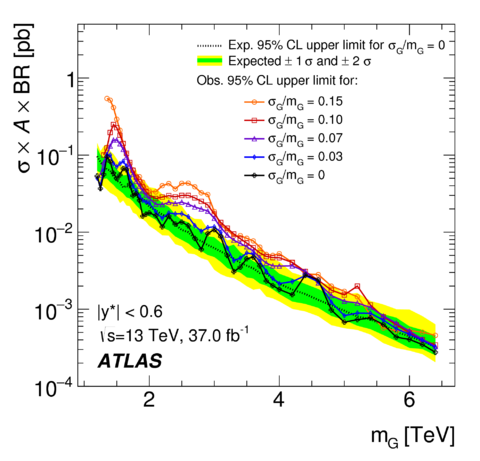
\includegraphics[width=0.8\columnwidth]{figures/Results/GaussianLimit.png}
%	\caption{The 95\% CL upper limits obtained from the dijet invariant mass $m_{jj}$ distribution on cross-section times acceptance times branching ratio to two jets, $\sigma \times A \times BR$, for a hypothetical signal with a cross-section $\sigma_G$ that produces a Gaussian contribution to the particle-level $m_{jj}$ distribution, as a function of the mean of the Gaussian mass distribution $m_G$. Observed limits are obtained for five different widths, from a narrow width to 15\% of $m_G$. The expected limit and the corresponding $\pm1\sigma$ and $\pm2\sigma$ bands are also indicated for a narrow-width resonance.
%}
%	\label{fig:GaussianLimit}
%\end{figure}